\chapter{Skills Analysis} % Main chapter title

\label{Chapter3} % Change X to a consecutive number; for referencing this chapter elsewhere, use \ref{Chapter3}

\lhead{Chapter 3. \emph{Skills Analysis}} % Change X to a consecutive number; this is for the header on each page - perhaps a shortened title

In this chapter I describe, analyse and demonstrate the knowledge and skills I have developed and gained throughout my university education
(see courses in Table~\ref{tbl:courses})
and work experiences in industry
(see placements in Figure~\ref{timeline}).
This has been done in line with the learning outcomes (LOs) as stipulated by the Engineering Council for the university programmes that the council accredits (see Appendix~\ref{App:ECLOs}), as well as the Graduate Attributes of Heriot-Watt University (see Appendix~\ref{App:HWgrad}).


% Please add the following required packages to your document preamble:
% \usepackage{booktabs}
% \usepackage{multirow}
\begin{table}[htbp]
	\caption{The courses I took for MEng Architectural Engineering}
	\label{tbl:courses}
	\centering
	\begin{tabular}{@{}lll@{}}
		\toprule
		\textbf{} & \textbf{Code} & \textbf{Course Title} \\ \midrule
		\multirow{8}{*}{\textbf{Year 1}} & D37TA & Construction Technology 1 \\
		& D17HH & History of the Built Environment \\
		& D17DE & Introduction to Design \\
		& F17XA & Mathematics for Engineers and Scientists 1 \\
		& D18BT & Building Services Technology \\
		& D27MB & Mechanics B \\
		& D47IE & Introduction to the Environment \\
		& F17XB & Mathematics for Engineers and Scientists 2 \\ \midrule
		\multirow{8}{*}{\textbf{Year 2}} & D18PA & Design Project A \\
		& D38TA & Construction Technology 2 \\
		& D18AB & Acoustics and Architectural Design \\
		& D28HA & Hydraulics and Hydrology A* \\
		& D17BG & Environment and Behaviour \\
		& F78SC & Statistics for Science \\
		& D18EP & Energy Principles and Applications \\
		& D18DP & Design Project B* \\ \midrule
		\multirow{8}{*}{\textbf{Year 3}} & D19CX & Critical Architectural Studies \\
		& D19EL & Electrical and Lighting Services for Buildings \\
		& D19SO & Design Software Applications \\
		& D39PZ & Procurement and Contracts \\
		& D19EB & Energy and Buildings \\
		& D19TP & Thermal Performance Studies \\
		& D19DI & Design Issues \\
		& D38FM & Facilities Management Principles \\ \midrule
		\multirow{6}{*}{\textbf{Year 4}} & D10YD/F & Design Project (AE) (S1/S2) \\
		& D10ZA/B & Dissertation (AE) (S1/S2) \\
		& D10LP & Laboratory Project \\
		& D10IE & Inclusive and Safe Environments \\
		& D10IS & Sustainable and Intelligent Buildings \\
		& D30IC & Innovation in Construction Practice \\ \midrule
		\multirow{7}{*}{\textbf{Year 5}} & D11PJ & Industrial Project \\
		& D11CA & Climate Change, Sustainability and Adaptation* \\
		& D21WC & Water Supply and Drainage for Buildings* \\
		& \textcolor{gray}{D11AF} & \textcolor{gray}{Architectural Acoustics} \\
		& \textcolor{gray}{D11DC} & \textcolor{gray}{Design of Low Carbon Buildings} \\
		& \textcolor{gray}{D11TH} & \textcolor{gray}{Thermofluids} \\
		& \textcolor{gray}{--} & \textcolor{gray}{\textit{To be determined}*} \\ \bottomrule
		\multicolumn{3}{l}{\textit{*Optional courses}} \\
		\multicolumn{3}{l}{\textcolor{gray}{\textit{Courses to be taken in 2019 are displayed in grey}}} \\
	\end{tabular}
\end{table}


I am studying an integrated Master of Engineering (MEng) degree in Architectural Engineering at Heriot-Watt University.
The degree is accredited by the Chartered Institution of Building Services Engineers (CIBSE), which is a licensed institution of the Engineering Council.
This means that when somebody joins CIBSE, they will also be registered as a Chartered Engineer (CEng), Incorporated Engineer (IEng) or Engineering Technician (EngTech) when they have reached the appropriate level of qualification and professional skill \citep{whyjoinCIBSE}.

The LOs of the degree programmes accredited by the Engineering Council are divided up into six categories:
\begin{itemize}
    \item Science and mathematics (SM)
    \item Engineering analysis (EA)
    \item Design (D)
    \item Economic, legal, social, ethical and environmental context (EL)
    \item Engineering practice (P)
    \item Additional general skills (G)
\end{itemize}
Each category has a list of LOs which are depicted by the category abbreviation (e.g. SM) and a number (e.g. 1); examples of LOs are SM1, EA2 and D3.
Most of these LOs are divided into, at the most, three incrementally increasing attainment levels which are depicted by the letters ``i", ``b" or ``m", e.g. SM1i, SM1b and SM1m.
From the \textit{UK Standard for Professional Engineering Competence} \hl{cite EC},
%\citep{EngineeringCouncil2014}, 
I have been able to deduce that:
\begin{itemize}
    \item \textbf{``i"} represents the LOs of Bachelors Degrees and Bachelors (Honours) Degrees accredited for IEng registration.
    \item \textbf{``b"} represents the LOs of Bachelors (Honours) Degrees accredited as partially meeting the educational requirement for CEng registration.
    \item \textbf{``m"} represents the LOs of integrated Masters (MEng) degrees accredited for CEng registration.
\end{itemize}

Some LOs are only divided into two attainment levels, one of which is not depicted by a letter ``i", ``b" or ``m", e.g. EA2i and EA2.
In such cases, the LO with the letter ``i", ``b" or ``m" applies to the corresponding attainment level and the LO without the letter applies to all the other attainment levels.
In the example of EA2i and EA2, EA2 applies to both attainment levels ``b" and ``m".

Other LOs, however, are not depicted by any of the letters ``i", ``b" or ``m", e.g. D6.
These LOs therefore apply to all three of the attainment levels.\footnote{
For consistency, I have amended seven of the LO abbreviations given to us in the D11PJ Course Handbook.
The LOs D3, EL3, EL6, P2, P11 and G3 were respectively changed to D3i, EL3b, EL6b, P2b, P11b and G3b.
Since the LOs P4 and P4m are identical, I have merged them to the single LO P4.
These amendments were done so that the naming conventions described above always apply.}

The approach of my skills analysis in this chapter is competency-based.
I have grouped the attainment levels of the LOs, such as SM1(i, b, m) and EA2(i, -), where the dash ``-" depicts the LO without ``i", ``b" or ``m" as an ending letter.
%\hl{Continue with the method I have used to demonstrate my achievement (or not) of the LOs, e.g. boxes for course codes.}

The \textit{UK Standard for Professional Engineering Competence} uses the following terms and their definitions, which will also apply within this document
%\citep{EngineeringCouncil2014}
\hl{Re-arranged extract from AHEP 3rd edition}:
\begin{itemize}
    \item \textbf{Awareness} is general familiarity, albeit bounded by the needs of the specific discipline

    \item \textbf{Knowledge} is information that can be recalled

    \item \textbf{Understanding} is the capacity to use concepts creatively, for example, in problem solving, design, explanations and diagnosis

    \item \textbf{Skills} are acquired and learned attributes that can be applied almost automatically

    \item \textbf{Know-how} is the ability to apply learned knowledge and skills to perform operations intuitively, efficiently and correctly

    \item \textbf{Complex} implies engineering problems, artefacts or systems that involve dealing simultaneously with a sizeable number of factors that interact and require deep understanding, including knowledge at the forefront of the discipline, to analyse or deal with

\end{itemize}


\begin{comment}
% Please add the following required packages to your document preamble:
% \usepackage{booktabs}
% \usepackage{multirow}
\begin{table}[h]
\caption{The courses I took towards my MEng degree in Architectural Engineering at Heriot-Watt University (include course codes? transpose table!)}
\label{courses}
	\begin{tabular}{@{}lp{8cm}p{7.5cm}@{}}
		\toprule
		& Semester 1 & Semester 2 \\ \midrule
		\multirow{4}{*}{\rot{Year 1}} & \textbullet \hspace{0.5ex}Construction Technology 1 & \textbullet \hspace{0.5ex}Building Services Technology \\
		& \textbullet \hspace{0.5ex}History of the Built Environment & \textbullet \hspace{0.5ex}Mechanics B \\
		& \textbullet \hspace{0.5ex}Introduction to Design & \textbullet \hspace{0.5ex}Introduction to the Environment \\
		& \textbullet \hspace{0.5ex}Mathematics for Engineers and Scientists 1 & \textbullet \hspace{0.5ex}Mathematics for Engineers and Scientists 2 \\ \midrule
		\multirow{4}{*}{\rot{Year 2}} & \textbullet \hspace{0.5ex}Design Project A & \textbullet \hspace{0.5ex}Environment and Behaviour \\
		& \textbullet \hspace{0.5ex}Construction Technology 2 & \textbullet \hspace{0.5ex}Statistics for Science \\
		& \textbullet \hspace{0.5ex}Acoustics and Architectural Design & \textbullet \hspace{0.5ex}Energy Principles and Applications \\
		& \textbullet \hspace{0.5ex}\textit{Hydraulics \& Hydrology A} & \textbullet \hspace{0.5ex}\textit{Design Project B} \\ \midrule
		\multirow{4}{*}{\rot{Year 3}} & \textbullet \hspace{0.5ex}Critical Architectural Studies & \textbullet \hspace{0.5ex}Energy and Buildings \\ 
		& \textbullet \hspace{0.5ex}Procurement and Contracts & \textbullet \hspace{0.5ex}Thermal Performance Studies \\
		& \textbullet \hspace{0.5ex}Design Software Applications & \textbullet \hspace{0.5ex}Design Issues \\
		& \textbullet \hspace{0.5ex}Electrical and Lighting Services for Buildings & \textbullet \hspace{0.5ex}Facilities Management Principles \\ \midrule
		\multirow{4}{*}{\rot{Year 4}} & \textbullet \hspace{0.5ex}Design Project (S1) & \textbullet \hspace{0.5ex}Design Project (S2) \\
		& \textbullet \hspace{0.5ex}Dissertation (S1) & \textbullet \hspace{0.5ex}Dissertation (S2) \\
		& \textbullet \hspace{0.5ex}Laboratory Project & \textbullet \hspace{0.5ex}Sustainable and Intelligent Buildings \\
		& \textbullet \hspace{0.5ex}Inclusive and Safe Environments & \textbullet \hspace{0.5ex}Innovation in Construction Practice \\ \midrule
		\multirow{4}{*}{\rot{Year 5}} & \textbullet \hspace{0.5ex}Industrial Project & \textbullet \hspace{0.5ex}Architectural Acoustics \\
		& \textbullet \hspace{0.5ex}\textit{Water Supply \& Drainage for Buildings} & \textbullet \hspace{0.5ex}Design of Low Carbon Buildings \\
		& \textbullet \hspace{0.5ex}\textit{Climate Change, Sustainability \& Adaptation} & \textbullet \hspace{0.5ex}Thermofluids \\
		&  & \textbullet \hspace{0.5ex}\textit{OPTIONAL} \\ \bottomrule
	\end{tabular}
\end{table}
\end{comment}



\begin{comment}
\begin{tcolorbox}[width=\textwidth/3,leftrule=3mm,enhanced,attach boxed title to top center={yshift=-3mm,yshifttext=-1mm},
colback=blue!5!white,colframe=blue!75!black,colbacktitle=red!80!black,
title=My title,fonttitle=\bfseries,
boxed title style={size=small,colframe=red!50!black} ]
This box uses a \textit{boxed title}. The box of the title can
be formatted independently from the main box.
\end{tcolorbox}
\end{comment}


%----------------------------------------------------------------------------------------
%	SECTIONS
%----------------------------------------------------------------------------------------

%----------------------------------------------------------------------------------------
%	SECTION 1
%----------------------------------------------------------------------------------------

\section{Science and Mathematics (SM)}

\subsection*{SM1(i, b, m)}

Multiple courses (mainly from years 2 and 3) have contributed to my knowledge and understanding of scientific principles and methodology necessary to underpin my education in Architectural Engineering.
A main contributor was \textit{Thermal Performance Studies}.
On this course I learned the scientific principles of psychrometrics, i.e. the properties of air-vapour mixtures (especially/ like air), and how to use this knowledge in the design of air conditioners, heat exchangers and cooling towers.
Learning about the environmental effects of refrigerants has contributed to my understanding of the evolution of air conditioners, from using carbon- and fluoride-based refrigerants to water and eventually phase change materials (PCMs) like Sunamp uses.

Learning the scientific principles of related disciplines has helped me enrich my appreciation of the scientific and engineering context of my discipline.
\textit{Statistics for Science} has, for example, helped me understand the proper methodology behind sampling populations and to identify bias in data.
\textit{Hydraulics and Hydrology A}, a civil engineering course, helped me appreciate the hydrological cycle (relevant to rainwater and urban drainage) and water flow in pipes (relevant to drainage, water supply and heating systems).


\subsection*{SM2(i, b, m)}

\textit{Mathematics for Engineers and Scientists 1 and 2} and \textit{Statistics for Science} all further developed my knowledge and understanding of mathematical and statistical methods.
I have been able to apply this knowledge in the analysis and solution of engineering problems.
For example, I used it to work out the yield of an array of photovoltaic panels (PV) in \textit{Energy and Buildings} as well as the yield of a set of turbines in a tidal energy generation system as part of my group project in \textit{Design Project}.


\subsection*{SM3(b, m)}

Other engineering disciplines that I have gained knowledge and understanding from are predominantly civil and structural.
These were acquired through the following courses: \textit{Mechanics B}, \textit{Construction Technology 1 and 2},  and \textit{Hydraulics and Hydrology A}.
%\hl{I cannot remember how I have applied or integrated this knowledge though...
%pipes?
%materials choice?}
I have been able to apply and integrate this knowledge and understanding to support study of my own engineering discipline, Architectural Engineering.
For example, during a \hl{CFD (1st time I mention CFD?)} modelling exercise in Laboratory Project, I was able to identify laminar and turbulent flows, something I had learned about it in \textit{Hydraulics and Hydrology A}.
This enabled me to refine and improve my CFD model.


\subsection*{SM4m}

A range of courses increased my awareness of developing technologies relevant to Architectural Engineering and building services.
In \textit{Building Services Technology}, \textit{Energy and Buildings}, \textit{Dissertation} and \textit{Innovation in Construction Practice}, I respectively learned about technologies such as modern windcatchers, smart meters, Building Information Modelling (BIM) and virtual and augmented reality.
I was also exposed to a developing technology during my placement at Sunamp: their heat batteries.
\hl{refer to work done at Sunamp?}


\subsection*{SM5m}

\hl{Is this skill about software???}
\textit{Design Software Applications} and \textit{Laboratory Project} enabled me to gain a comprehensive knowledge and understanding of software used by architectural engineers.
I learned how steady-state and dynamic software applications function, was made aware of the mathematical \hl{models/ formulas} they are based on and learned about their limitations.
\hl{Should I give examples of limitations to demonstrate my knowledge/ understanding? Not necessarily part of marking criteria.}
I was introduced to and got to practise using the following applications:
\begin{itemize}
    \item Steady-state: iSBEM (an interface for Simplified Building Energy Model), SAP (Standard Assessment Procedure) and PHOENICS (a CFD software application)
    \item Dynamic: IES-VE (Integrated Environmental Solutions - Virtual Environment)
    \item Computational fluid dynamics (CFD): PHOENICS?
\end{itemize}

% Please add the following required packages to your document preamble:
% \usepackage{booktabs}
\begin{table}[htbp]
\begin{tabular}{@{}lp{8cm}@{}}
\toprule
Type of software & Applications \\ \midrule
Steady-state & iSBEM (an interface for Simplified Building Energy Model) \\
 & SAP (Standard Assessment Procedure) \\
 & PHOENICS (a CFD software application) \\
Dynamic & IES-VE (Integrated Environmental Solutions - Virtual Environment) \\
Computational fluid dynamics (CFD)? & PHOENICS? \\ \bottomrule
\end{tabular}
\end{table}

\hl{List or table?}

\hl{Although it is outside the scope of this learning outcome, I would like to add that these courses did not allow me to properly develop my skills in using the software...}


\subsection*{SM6m}

\hl{How does this fall under Science and Maths heading?}

I have been able to critically evaluate and apply a range of concepts, including some outside engineering, in my engineering projects.
\hl{EXAMPLE 1:}
I learned about the sustainable design hierarchy (see Figure~\ref{fig_hierarchy}) during my placement at Arup.
I then applied this approach to the design of a library for a group project in \textit{Critical Architectural Studies}, helping us earn the first prize in Sustainable Design (see Figure~\ref{fig_award}).
\hl{EXAMPLE 2:}
Upon conducting a post-occupancy evaluation (POE) for \textit{Environment and Behaviour}, I came across a social sciences journal paper about survey research.
It analysed typical response styles and suggested how to design questionnaires to avoid biased or inaccurate data collection.
Using these \hl{criteria/ suggestions}, I was able to critically evaluate the success of the questionnaire used for the POE in \textit{Environment and Behaviour} and design an improved survey questionnaire for the acoustic \textit{Laboratory Project}.

\begin{figure}[htbp]
	\centering
	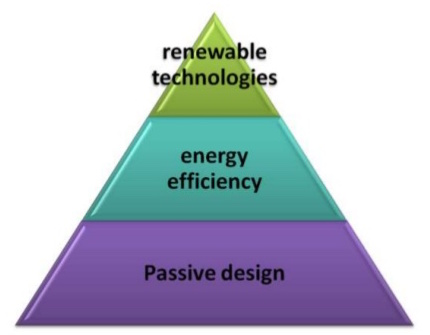
\includegraphics[width=10cm]{figures/Hierarchy.jpg}
	\rule{\textwidth}{0.5pt} % use line???
	\caption{The sustainable design hierarchy %\citep{Dougherty:online}.
	}
	\label{fig_hierarchy}
\end{figure}


\begin{figure}[htbp]
	\centering
	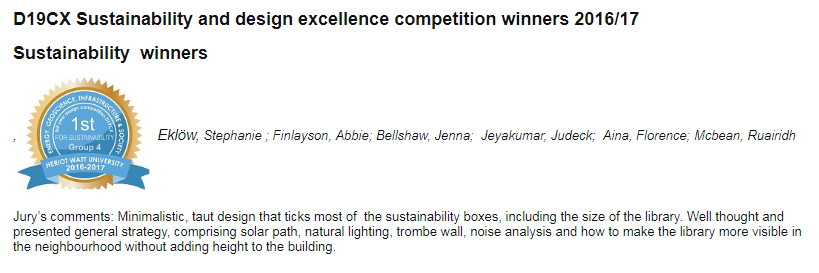
\includegraphics[width=\textwidth]{figures/SustainabilityAward.png}
	\rule{\textwidth}{0.5pt} % use line???
	\caption{First prize for sustainability awarded to my group for our library design in \textit{Critical Architectural Studies} (D19CX).}
	\label{fig_award}
\end{figure}

\hl{Other courses?}
\begin{itemize}
	\item Use of solar gain in pool house (\textit{first year collaborative project})?
	\item Contact factor in \textit{LAB CFD}?
	\item Learned in \textit{CAS}, applied again in \textit{y4 collab}: make design concept red thread...
\end{itemize}



%----------------------------------------------------------------------------------------
%	SECTION 2
%----------------------------------------------------------------------------------------

\section{Engineering Analysis (EA)} \label{EA}

\subsection*{EA1(i, b, m)} 

\begin{wraptable}{r}{0.2\textwidth}
	\begin{tabular}{|ll|}
		\hline
		\multicolumn{2}{|c|}{\cellcolor[HTML]{F8A102}\textbf{EA1(i, b, m) \nomaster}} \\ \hline
		\EPA & \DSA \\
		\TPS & \LAB \\ \hline
	\end{tabular}
\end{wraptable}

In some courses, I have conducted laboratory experiments and modelling exercises.
This has further developed my skills in monitoring, interpreting and applying the results of analysis and modelling to bring about continuous improvement [EA1i].
\textit{Laboratory Project} went a step further and taught me the principles and process to engineering a better solution [EA1b and EA1m].
These principles were applied in an engineering project which aimed to optimise the design of a cooling coil.
Having earned As on all of the courses listed in the course box shows that I have an understanding of engineering principles and the ability to apply them to analyse key engineering processes.







\newpage
\subsection*{EA2(i, -)}

\begin{wraptable}{r}{0.2\textwidth}
	\begin{tabular}{|ll|}
		\hline
		\multicolumn{2}{|c|}{\cellcolor[HTML]{F8A102}\textbf{EA2(i, -) \nomaster}} \\ \hline
		\ConTechOne & \Acoustics \\
		\HYD & \EPA \\
		\TPS & \PRJ \\
		\LAB &  \\
		Arup & Sweco \\ \hline
	\end{tabular}
\end{wraptable}

A range of courses have developed my ability to understand and explain the performance of systems and components through the use of quantitative/ analytical methods and/ or modelling techniques.
For example, in \textit{Hydraulics and Hydrology A}, I learned how to use quantitative methods to distinguish laminar flows from turbulent flows.
And when we were studying thermofluids in \textit{Laboratory Project}, I used both CFD modelling and analytical methods to understand and describe the performance of a cooling coil in an air conditioning unit.

I have also applied quantitative/ analytical methods and/ or modelling techniques to classify and describe the performance of systems during my work placements at Arup and Sweco.
In particular, at Sweco I used a combination of the aforementioned methods and techniques to describe the performance of some buildings in terms of solar heat gain, energy consumption, thermal comfort, and daylighting.
The results of these analyses were then classified according to the criteria of \textit{Miljöbyggnad}: Gold, Silver, Bronze or Disapproved (see Figure~\ref{fig:svl}).








\subsection*{EA3(i, b, m)} \label{EA3}

\begin{wraptable}{r}{0.2\textwidth}
	\begin{tabular}{|ll|}
		\hline
		\multicolumn{2}{|c|}{\cellcolor[HTML]{F8A102}\textbf{EA3(i, b, m) \nomaster}} \\ \hline
		\MechB & \HYD \\
		\DPB & \DSA \\
		\EnBldgs & \TPS \\
		\PRJ & \LAB \\ \hline
	\end{tabular}
\end{wraptable}

I have developed the ability to use the results of analysis and apply quantitative and computational methods to solve engineering problems and subsequently recommend or implement appropriate action in some courses.
For example, a combination of calculations, CFD modelling and a physical laboratory experiment were used to optimise the design of a cooling coil in \textit{Laboratory Project}.
This was an iterative process of solving problems and implementing appropriate actions to come up with a better solution, for which I earned an A.
However, I do not think I have ever used alternative approaches to solve engineering problems and implement appropriate action [EA3m]; this is a skill I need to develop.







\subsection*{EA4(i, b, m)}

\begin{wraptable}{r}{0.2\textwidth}
	\begin{tabular}{|ll|}
		\hline
		\multicolumn{2}{|c|}{\cellcolor[HTML]{F8A102}\textbf{EA4(i, b, m) \nomaster}} \\ \hline
		\CAS & \EnBldgs \\
		\PRJ & \WSD \\ \hline
	\end{tabular}
\end{wraptable}

Some courses have contributed to my understanding of, and ability to apply, an integrated or systems approach to solving complex engineering problems through know-how of the relevant technologies and their application.
I would not say this skill is fully developed though as I have not had many opportunities to develop it.
An example of when I did fully demonstrate my ability to achieve LOs EA4i, EA4b and EA4m is my natural lighting design of Newington Library in \CASTitle.
With the aim of maximising daylight and avoiding direct sunlight, I had to take several aspects into consideration in the fenestration design:
\begin{itemize}
	\item The building orientation and sun path
	\item The characteristics and desirability of the natural light hitting each fa{\c{c}}ade
	\item Functions of the internal and external spaces and their required lighting levels
	\item Type of glazing (double/ triple, clear/ frosted)
	\item Subsequent thermal comfort and energy loads related to the choice of glazing
\end{itemize}


I will give an example to demonstrate the interdependent nature of this design exercise.
The south-west corner of the library housed a shelving and study area.
However, the south-west fa{\c{c}}ade would be receiving an intense afternoon sunlight, which was undesirable due to glare and the sunlight's detrimental effects on the books.
I therefore designed clerestory glazing to (a) limit direct incoming sunlight, (b) exclude distracting, unattractive or intrusive views, and (c) allow shelving against wall (see Figure~\ref{fig:nl}).
Additionally, the clerestory glazing was frosted to disperse the sunlight's rays.
My natural lighting design was commended by the judges of the course's design competition (see Figure~\ref{fig_award}).


\begin{figure}[htbp]
	\centering
	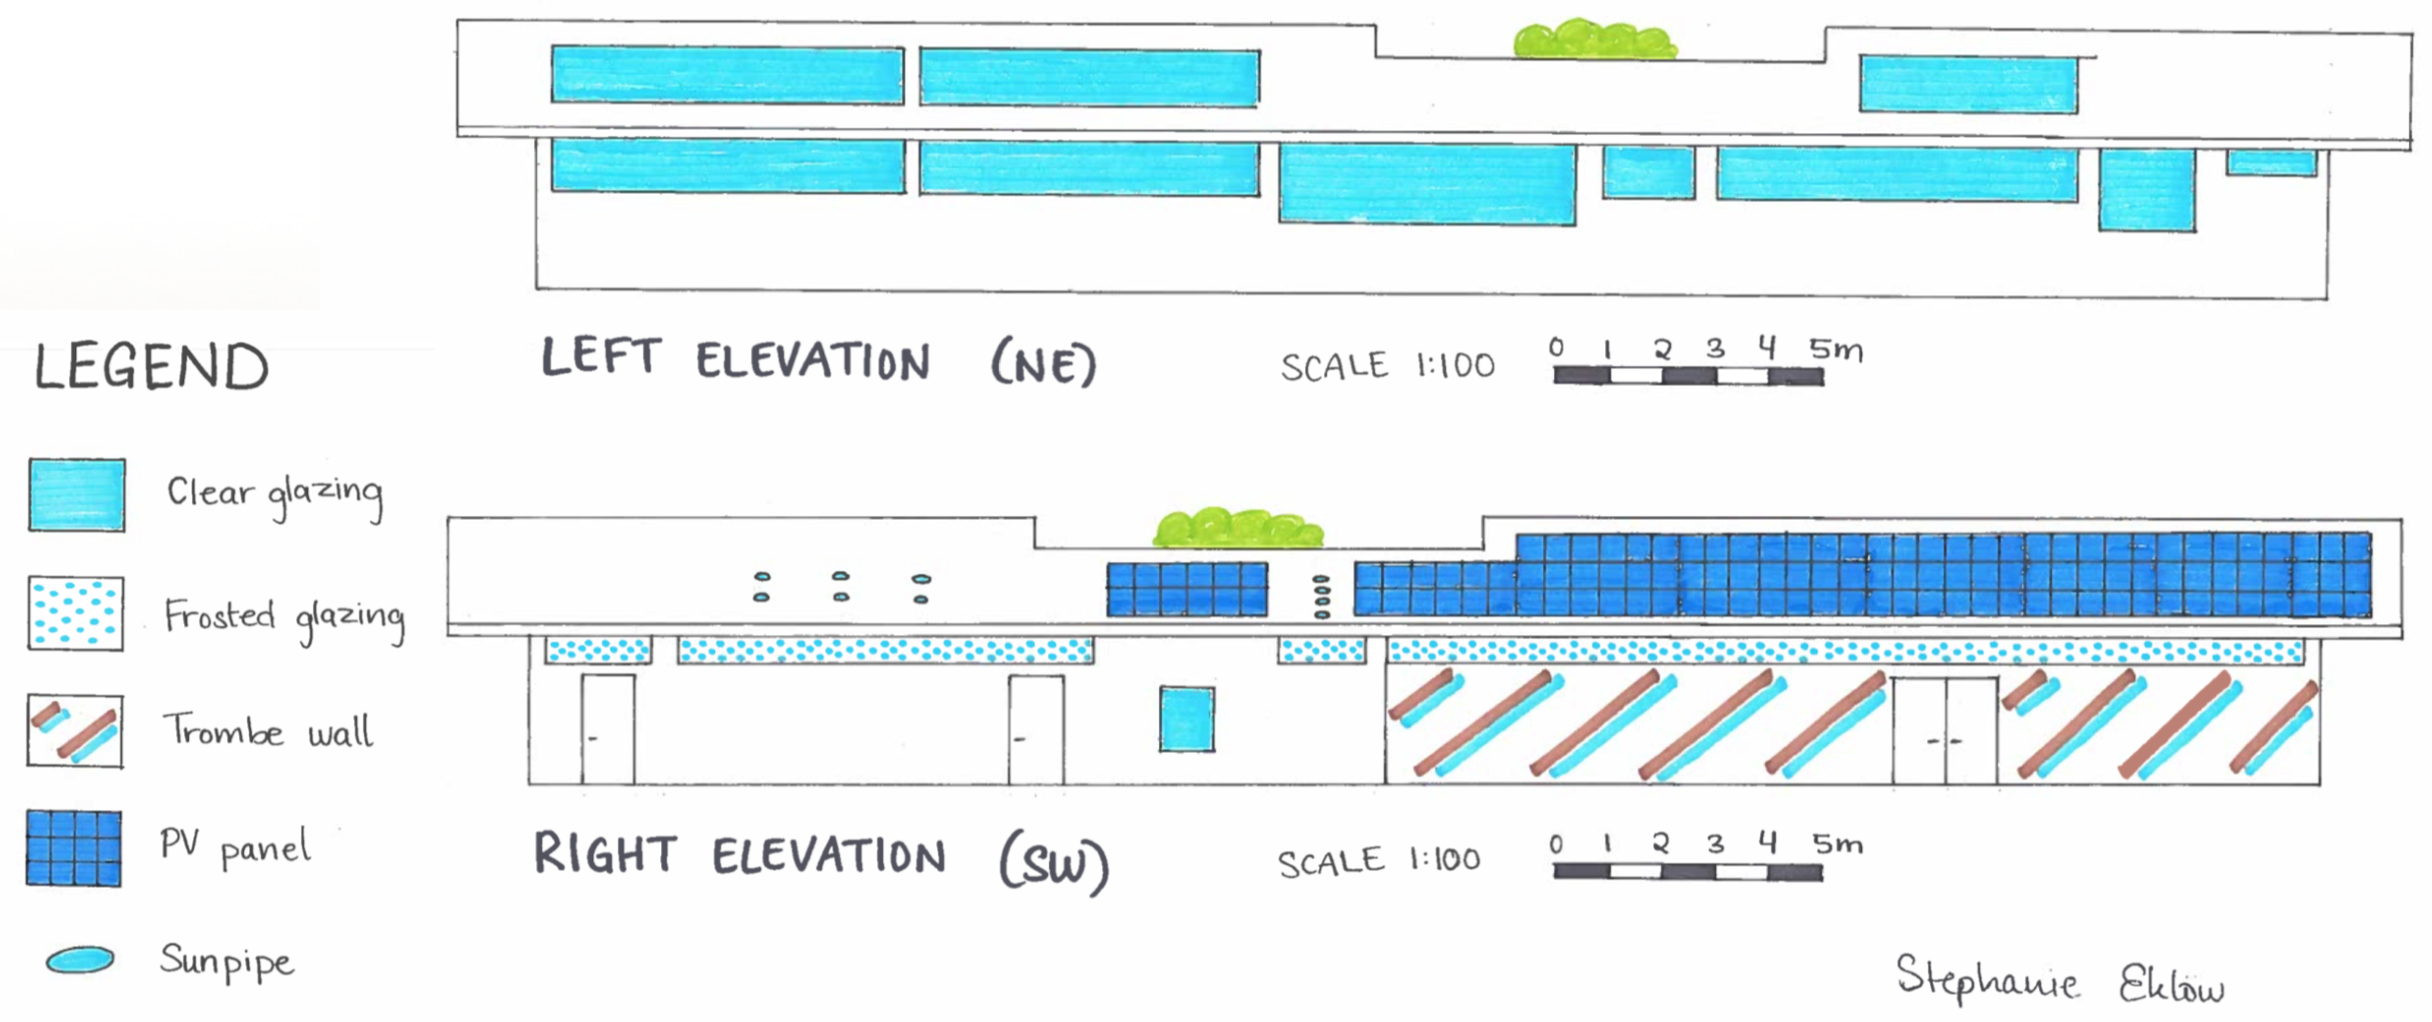
\includegraphics[width=\textwidth]{figures/NL-nl.png}
	\rule{\textwidth}{0.5pt} % use line???
	\caption{The fit-for-purpose glazing scheme of Newington Library.}
	\label{fig:nl}
\end{figure}

%\hl{If I look overll at all the steps (integrated), I can go down that path. but if I just look at the step that isn't working, I'd go down another path. Look at something that wasn't working, and . CCSA eposter: not to miss point of question/ topic (how to harness lessons from past climate events); focusing on other parts of question sets us up to fail. Because I know about this, I can apply it to engineering in the following ways. Sunamp PISs. Made sure whole process was more carefully thought out than it was when I was given the job. I had an overview of the whole thing. I made sure that the document enabled people to use the batteries as efficiently as possible. Can't do that by looking at each point of its own - it's got to flow as a document. specific application of heat batteries  - know-how  of technology and application (0.5 page)}








\newpage
\subsection*{EA5m}

\begin{wraptable}{r}{0.2\textwidth}
	\begin{tabular}{|ll|}
		\hline
		\multicolumn{2}{|c|}{\cellcolor[HTML]{F8A102}\textbf{EA5m \master}} \\ \hline
		\EnBldgs & \PRJ \\
		\DST & \ICP \\
		Hoare Lea & Sunamp \\ \hline
	\end{tabular}
\end{wraptable}

Some courses and placements have enabled me to develop my ability to use fundamental knowledge to investigate new and emerging technologies.
My most extensive investigation is of Sunamp's heat batteries, having developed the PISs and a Product Selection Quiz for their UniQ product range (see Appendices~\ref{App:PISs} and \ref{App:quiz}).
My knowledge of heat exchangers (gained notably in the thermofluids part of the \LABTitle),
water supply and heating (gained in the \PRJTitle),
and renewable technologies (gained in \EnBldgsTitle)
contributed to my understanding of the operation of Sunamp's heat batteries.










\subsection*{EA6m} \label{sec:EA6m}

\begin{wraptable}{r}{0.2\textwidth}
	\begin{tabular}{|ll|}
		\hline
		\multicolumn{2}{|c|}{\cellcolor[HTML]{F8A102}\textbf{EA6m \littlemaster}} \\ \hline
		\multicolumn{2}{|c|}{\PRJ} \\ \hline
	\end{tabular}
\end{wraptable}

I do not have a lot of experience extracting and evaluating pertinent data to apply engineering analysis techniques in the solution of unfamiliar problems.
The only example I can think of is when I tried to calculate the yield of tidal power for the \textit{4th year collaborative project}, which was part of the \PRJTitle.
This was an unfamiliar problem and I could only find information online on how to calculate yields from hydroelectric dams.
Thus, I had to use a combination of the information I found, assumptions and my own fundamental mathematical skill set.
I found that four bi-directional turbines with a total of four ebb and flood tides of three metres could generate a daily total of 284~kWh, but this was only 16\% of the building's daily electricity demand.
Since I never showed my workings to anyone, I cannot be sure if they were correct.
Overall, I believe I could use some more development in this skill area.

%----------------------------------------------------------------------------------------
%	SECTION 3
%----------------------------------------------------------------------------------------

\section{Design (D)}

\subsection*{D1(i, -)}

\begin{wraptable}{r}{0.2\textwidth}
	\begin{tabular}{|ll|}
		\hline
		\multicolumn{2}{|c|}{\cellcolor[HTML]{F8A102}\textbf{D1(i, -) \master}} \\ \hline
		\ID & \IE \\
		\EnvBeh & \CAS \\
		\ELS & \PC \\
		\FMP & \PRJ \\
		\ISE & Sunamp \\ \hline
	\end{tabular}
\end{wraptable}

Multiple courses have developed and contributed to my understanding and ability to evaluate business, customer and user needs.
The concept of a good brief that reflects the business, customer and user needs has been emphasised throughout the AE programme.
I have been able to evaluate such needs through various assignments and in different contexts, such as technical aspects (air quality, lighting levels and fire safety), users with different kinds of disabilities, and public perception.
During my placement at Hoare Lea, I was able to evaluate the design brief of a mixed-use new-build for needs regarding fire safety in order to design the fire detection and alarm systems.
Moreover, half of the marks for \CASTitle \space were based on a group project and our ability to respond to the design brief of Newington Library.
I cannot find the mark I got specifically for this project, but our group won first prize in sustainability (see Figure~\ref{fig_award}) and I got an overall A for that course.
I can thus deduce that I achieved LOs D1i and D1.

%Some of these courses considered more technical needs such as good air quality and lighting levels, which are dependent on the functions of spaces.
%In \textit{Procurement and Contracts} and \textit{Facilities Management Principles}, I learned about the different stakeholders involved in a project and their respective needs and interests.







\subsection*{D2(i, -)}

\begin{wraptable}{r}{0.2\textwidth}
	\begin{tabular}{|ll|}
		\hline
		\multicolumn{2}{|c|}{\cellcolor[HTML]{F8A102}\textbf{D2(i, -) \master}} \\ \hline
		\DI & \DST \\
		\LAB & \CCSA \\ \hline
	\end{tabular}
\end{wraptable}

I have developed the ability to define and investigate a problem in my later years at Heriot-Watt University.
For example, for \DITitle, we were required to write a short report on the impact of climate on an area of construction/ building services in a country of our own choice.
For this, I selected Guyana, a tropical country in South America.
A Guyanese local told me about the lack of shading on buildings in their country.
This was my starting point, from where I defined and investigated the problem.
I conducted a literature review that revealed the need for shading in tropical countries to help avoid overheating in buildings and reduce cooling energy loads.
Hence, a lack of shading in a tropical climate is problematic as overheating poses health risks to building occupants (e.g  heat stress and even death) and the increased use of air conditioners is not only expensive to run, but emits greenhouse gases, thus contributing to climate change.
I then proceeded to investigate the extent of the shading deficiency on Guyana's commercial buildings by conducting an evidence review.
This included examining Guyanese newspaper articles and speaking with a couple people from Guyana, one of whom is a local architect.
I was able to confirm the increasing lack of shading on modern commercial buildings and identify the reasons for this.
These include a lack of regulations on buildings and designers, and the appeal of the international glass-dominated architecture style (enabled due to technologies like air conditioning).

I have similarly defined and investigated problems for the \DSTTitle \space and in assignments for \LABTitle \space and \CCSATitle.
My marks for these assignments (one B and four As) demonstrate my full achievement of LOs D2i and D2.








\subsection*{D3(i, b, m)}

\begin{wraptable}{r}{0.2\textwidth}
	\begin{tabular}{|ll|}
		\hline
		\multicolumn{2}{|c|}{\cellcolor[HTML]{F8A102}\textbf{D3(i, b, m) \littlemaster}} \\ \hline
		\DPB & \PRJ \\
		\LAB &  \\
		Sunamp & Sweco \\ \hline
	\end{tabular}
\end{wraptable}

Working with information that may be incomplete or uncertain is something that I have found difficult.
\textit{Design Project B}, \textit{Design Project} and \textit{Laboratory Project} are courses that particularly challenged me in this area and helped me develop the skill.
During these projects I learned to make assumptions and use iterative/ trial-and-error processes to come up with a satisfactory design solution.
The fact that I passed all these courses demonstrates that I have some ability to work with incomplete or uncertain information.
%This was done, for example, for the sizing of pipes in the design projects.
However, I still consider my ability to do this to be rather weak.

I do not think I have ever gone as far as to quantify the effect of incomplete or uncertain information on a design and to use research to mitigate the deficiencies.
I need to develop these abilities as I presume they will be necessary in industry, where the information required to carry out design tasks may not always be certain or complete.








\subsection*{D4(i, -)}

\begin{wraptable}{r}{0.2\textwidth}
	\begin{tabular}{|ll|}
		\hline
		\multicolumn{2}{|c|}{\cellcolor[HTML]{F8A102}\textbf{D4(i, -) \nomaster}} \\ \hline
		\DPA & \DPB \\
		\CAS & \EnBldgs \\
		\PRJ &  \\ \hline
	\end{tabular}
\end{wraptable}

All of my design projects at Heriot-Watt University have developed my skills in creating design solutions that are fit for purpose through application of problem-solving skills, technical knowledge and understanding.
%\textit{1st year collaborative project},
%\textit{Design Project A},
%\textit{Design Project B},
%\textit{Critical Architectural Studies},
%\textit{Energy and Buildings},
%and \textit{Design Project}, including the \textit{4th year collaborative project}.
%\hl{Give examples?! However, I cannot think of an example where the whole life cycle was considered, especially disposal.}
For example, in \CASTitle, I ensured the lighting design of Newington Library was fit for purpose by helping determine the building orientation and the layout of the internal rooms, considering the possible overshadowing effect of neighbouring buildings and maximising daylighting.
My customised natural lighting design was commended in the design competition (see Figure~\ref{fig_award}).

I, however, have not established rigorous design solutions that are fit for purpose for \emph{all} aspects of the problem.
So far, I have only created bespoke solutions that considered one or some aspects of a building's life cycle, e.g. production, operation and/ or maintenance.
I cannot think of an example where I considered the demolition and disposal of a building.
Therefore, I have not accomplished LO D4.
Perhaps I will get the opportunity to create a `life cycle solution' in next semester's course \LCBTitle.









\subsection*{D5(i, -)}

\begin{wraptable}{r}{0.2\textwidth}
	\begin{tabular}{|ll|}
		\hline
		\multicolumn{2}{|c|}{\cellcolor[HTML]{F8A102}\textbf{D5(i, -)} \nomaster} \\ \hline
		\IE & \DPA \\
		\DPB & \CAS \\
		\PRJ & \DST \\
		\LAB & \CCSA \\ \hline
	\end{tabular}
\end{wraptable}

I have had some experience in planning and managing design processes, notably in group design projects (whether it was the design of a building or a poster \ldots).
I have also evaluated the outcomes of a design process, notably in a reflective report submitted after the design of a library in \CASTitle.
Some reflective points from that report (on which I got an A$+$) on what makes a good design process are \citep{eklowCAS}:
\begin{itemize}
	\item ``a strong concept [\ldots] helped guide us through all of our decision-making and eventually come up with a good-quality design"
	\item ``The final group design could have been improved [\ldots] if the building solution had been finalised earlier [\ldots]. This could have been achieved by planning the design timeline right from the start, something we failed to do."
	\item ``I learned that tasks should be sized and assigned according to each individual’s commitment/ reliability" rather than in fairness.
\end{itemize}

I have, however, never planned or managed the cost drivers of a design process, despite having had opportunities to do this.
The task of costing was either allocated to another group member, or (as was the case for the \PRJTitle) I failed to do it due to poor time management.







\subsection*{D6}

\begin{wraptable}{r}{0.2\textwidth}
	\begin{tabular}{|ll|}
		\hline
		\multicolumn{2}{|c|}{\cellcolor[HTML]{F8A102}\textbf{D6 \master}} \\ \hline
		\DPA & \ConTechOne \\
		\HYD & \EnvBeh \\
		\DPB & \CAS \\
		\TPS & \DI \\
		\FMP & \PRJ \\
		\DST & \LAB \\
		\ISE & \CCSA \\
		Sunamp & Sweco \\ \hline
	\end{tabular}
\end{wraptable}

Most of the assignments I have written and presentations I have given contributed to the development of my skill of communicating to technical or non-technical audiences.
Instances of communicating to non-technical audiences include my POSTnote assignment for \textit{Climate Change, Sustainability and Adaptation}, where I wrote about a technical topic to members of the UK parliament (see more under the second bullet point in Section~\ref{sec:G1}), and the UniQ PISs that I created for Sunamp which needed to convey the technical operation of their products in layman's terms.
Most laboratory reports I have written, e.g. for \textit{Laboratory Project}, were of a technical nature.
To name a few, my provisional grade of B in the POSTnote and my final grades of A in the laboratory reports demonstrate my accomplishment of LO D6.







\subsection*{D7m}

\begin{wraptable}[9]{r}{0.2\textwidth}
	\begin{tabular}{|ll|}
		\hline
		\multicolumn{2}{|c|}{\cellcolor[HTML]{F8A102}\textbf{D7m \nomaster}} \\ \hline
		\ConTechOne & \ID \\
		\EnvBeh & \CAS \\
		\PC & \FMP \\
		\PRJ & \DST \\
		\LAB & \SIB \\
		\ICP & Arup \\
		H{\&}L & Hoare Lea \\ \hline
	\end{tabular}
\end{wraptable}

Multiple courses and work placements have contributed to my wide knowledge and comprehensive understanding of design processes and methodologies.
\PC, amongst other courses, has exposed me to various building design and construction procurement routes and processes, particularly the RIBA Plan of Work 2013.
The thermofluids part of \textit{Laboratory Project} taught me about the methodology for optimising a design.
This knowledge has been complemented by information about specific parts of the design process, such as the briefing stage, site analysis, POEs and life cycle assessments.
%UK vs Sweden: Arup, 
%HL, FMP, DST, P\&C vs H\&L
%BIM: DST, ICP
%Engineering optimisation: LAB
%From site analysis to POEs + LCA: Con tech 1, Intro to Design, Env and Beh, SIB
I have also delved into a study of BIM, a new way to approach collaborative building design which is the new ``Holy Grail" of design processes, during the \DSTTitle.
The fact that I received an overall A grade in the three aforementioned courses demonstrates my knowledge and understanding of design processes and methodologies.

Furthermore, I have developed an ability to apply and adapt these design processes and methodologies in unfamiliar situations.
For example, the \PRJTitle \space comprised of two stages which resembled Stages 2 (Concept Design) and 3 (Developed Design) of the RIBA Plan of Work 2013.
And in \CASTitle, I took the initiative to conduct a site analysis and develop a POE questionnaire to improve the design of the library.
Having passed both courses proves my ability to apply and adapt design processes and methodologies in unfamiliar situations.








\subsection*{D8m}

\begin{wraptable}{r}{0.2\textwidth}
	\begin{tabular}{|ll|}
		\hline
		\multicolumn{2}{|c|}{\cellcolor[HTML]{F8A102}\textbf{D8m} \nomaster} \\ \hline
		\PRJ & Sunamp \\ \hline
	\end{tabular}
\end{wraptable}

The way that I developed the UniQ Product Selection Quiz (described in Section~\ref{sec:quiz}) is a demonstration of my ability to generate an innovative design for products, systems, components or processes to fulfil new needs.
I also came up with the innovative idea of generating tidal power for the 4\textsuperscript{th} year collaborative project (described in Section~\ref{sec:P10m}), but this was not fully designed.
Since I have not created many innovative designs to fulfil new needs, I would not say that I have fully developed or mastered this skill.



%----------------------------------------------------------------------------------------
%	SECTION 4
%----------------------------------------------------------------------------------------

\section{Economic, Legal, Social, Ethical and Environmental Context (EL)}

\subsection*{EL1(-, m)}

I gained an understanding of the need for a high level of professional and ethical conduct in engineering and a knowledge of professional codes of conduct in \textit{Procurement and Contracts}.
I familiarised myself with CIBSE's and \hl{...} professional codes of conduct in an assignment where \hl{...}
This course and my ethical induction at Arup also taught me how ethical dilemmas can arise.
\hl{Elaborate?}





\subsection*{EL2}

\begin{wraptable}{r}{0.2\textwidth}
	\begin{tabular}{|ll|}
		\hline
		\multicolumn{2}{|c|}{\cellcolor[HTML]{F8A102}\textbf{EL2}} \\ \hline
		\ID & \DI \\
		\DST & \SIB \\
		Sunamp &  \\ \hline
	\end{tabular}
\end{wraptable}


I have gained knowledge and understanding of the commercial, economic and social context of engineering processes.
A pertinent example which touches all of these aspects is one that I gave in a debate in \IDTitle \space after having heard about it from Stuart MacPherson, the owner of Irons Foulner Consulting Engineers.
Around 2002, Stuart had been appointed to design or refurbish the building services of the Queen's Gallery in Edinburgh (see Figure~\ref{fig:qg}).
Rather than taking the most energy efficient and sustainable approach to the design, he had to consider the social and commercial context of the gallery.
One of the requirements was that none of the services could be visible, as this would not look attractive to the visitors.
Another requirement was that the temperature and humidity levels needed to be maintained within strict ranges so that the artwork would not get damaged.
This is challenging considering that flows of people would be coming in and out of the gallery, possibly with their wet coats and umbrellas on rainy days, causing heat and humidity to constantly be exchanged with the outdoors and the visitors themselves.
In order to isolate the artwork from its environment, so to speak (see Figure~\ref{fig:isolation}), Stuart had to have sensors installed that would detect fluctuations in temperature and humidity, as well as precise ventilation and heating systems that would constantly maintain the acceptable ranges.
This would consequently make the project more expensive, but it was considered necessary for the running of the gallery.

\begin{figure}[htbp]
	\centering
	\begin{subfigure}[b]{0.5\textwidth}
		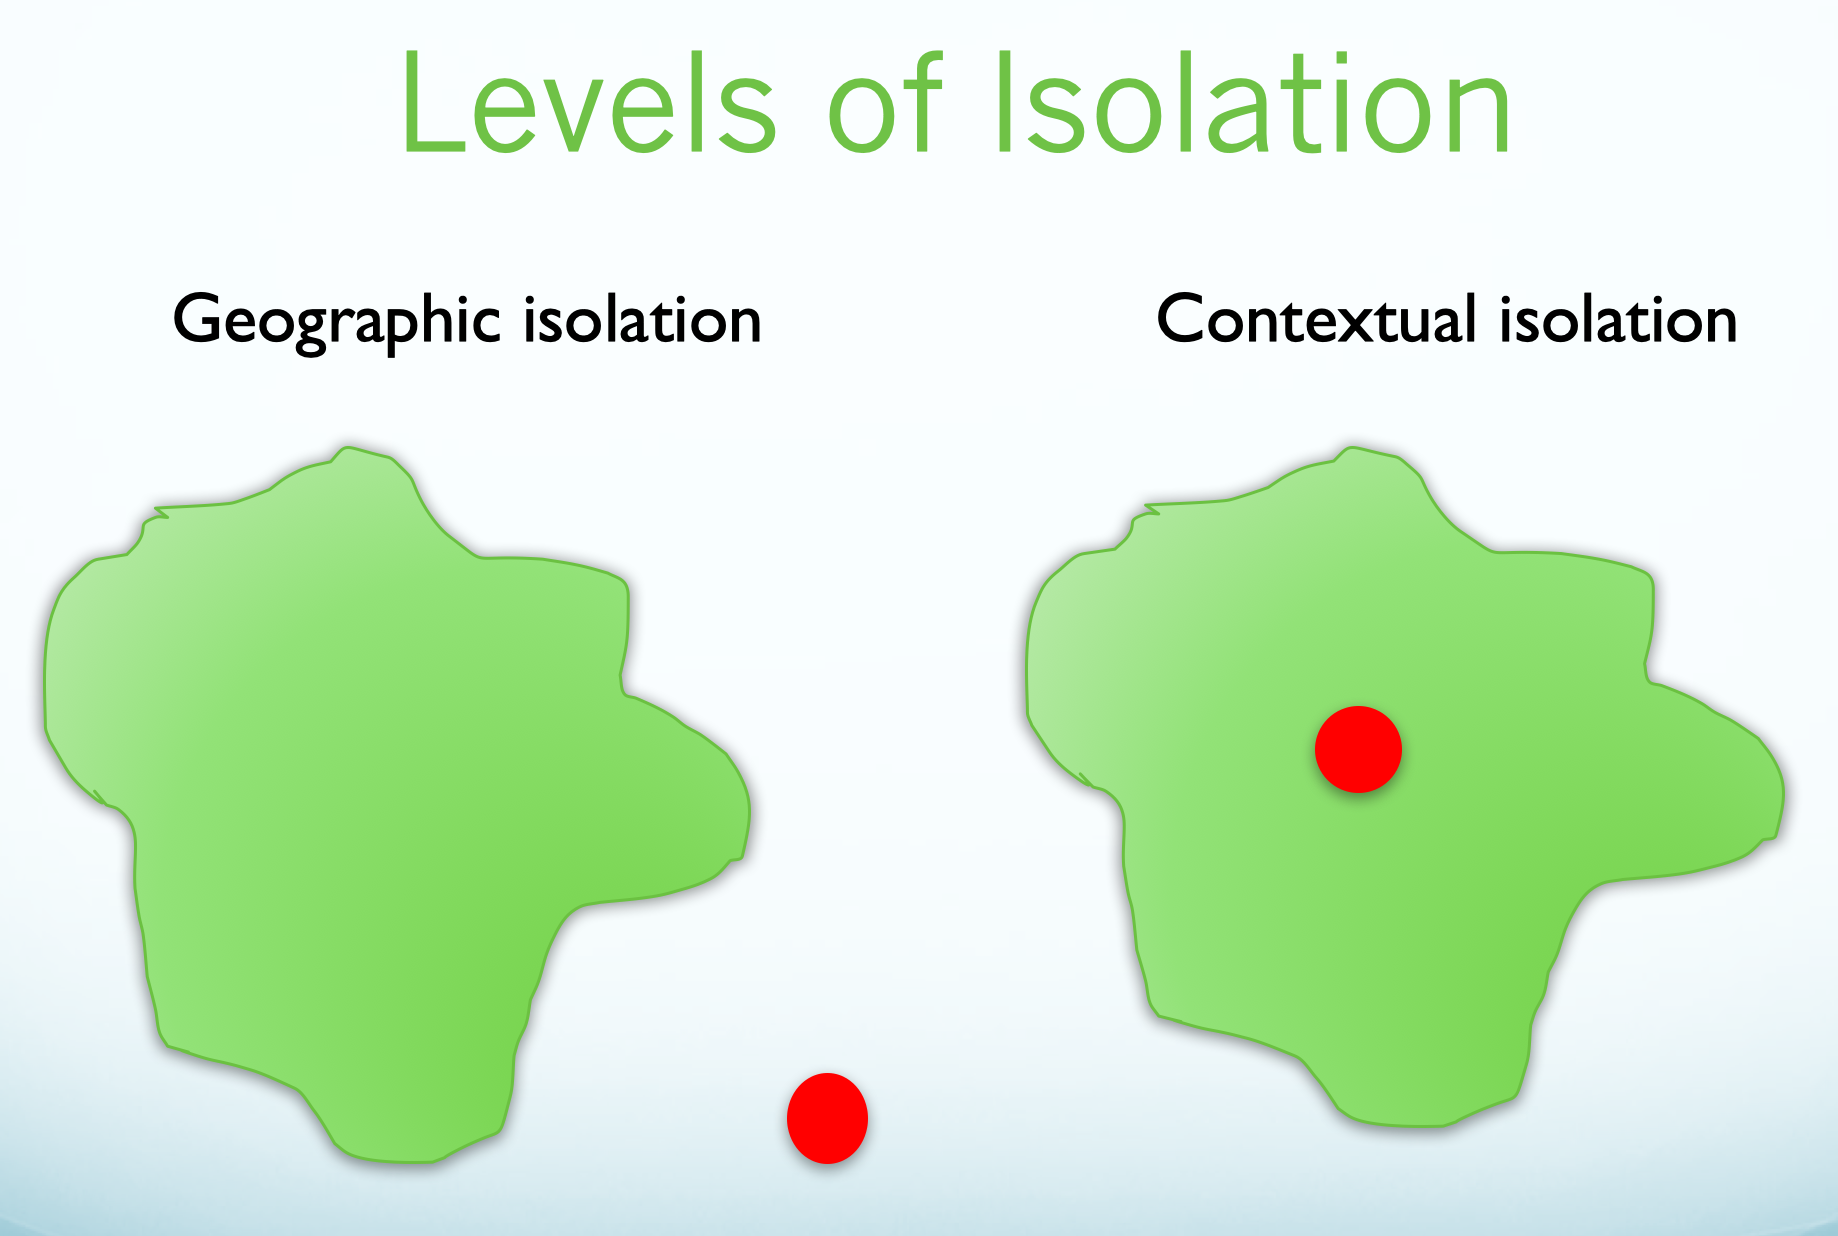
\includegraphics[width=\textwidth]{figures/isolation.png}
		\caption[Contextual isolation.]{A graphical representation of contextual isolation that I created and used in a PowerPoint for a group debate in \ID}\label{fig:isolation}
	\end{subfigure}
	
	\begin{subfigure}[b]{.48\textwidth}
		\centering
		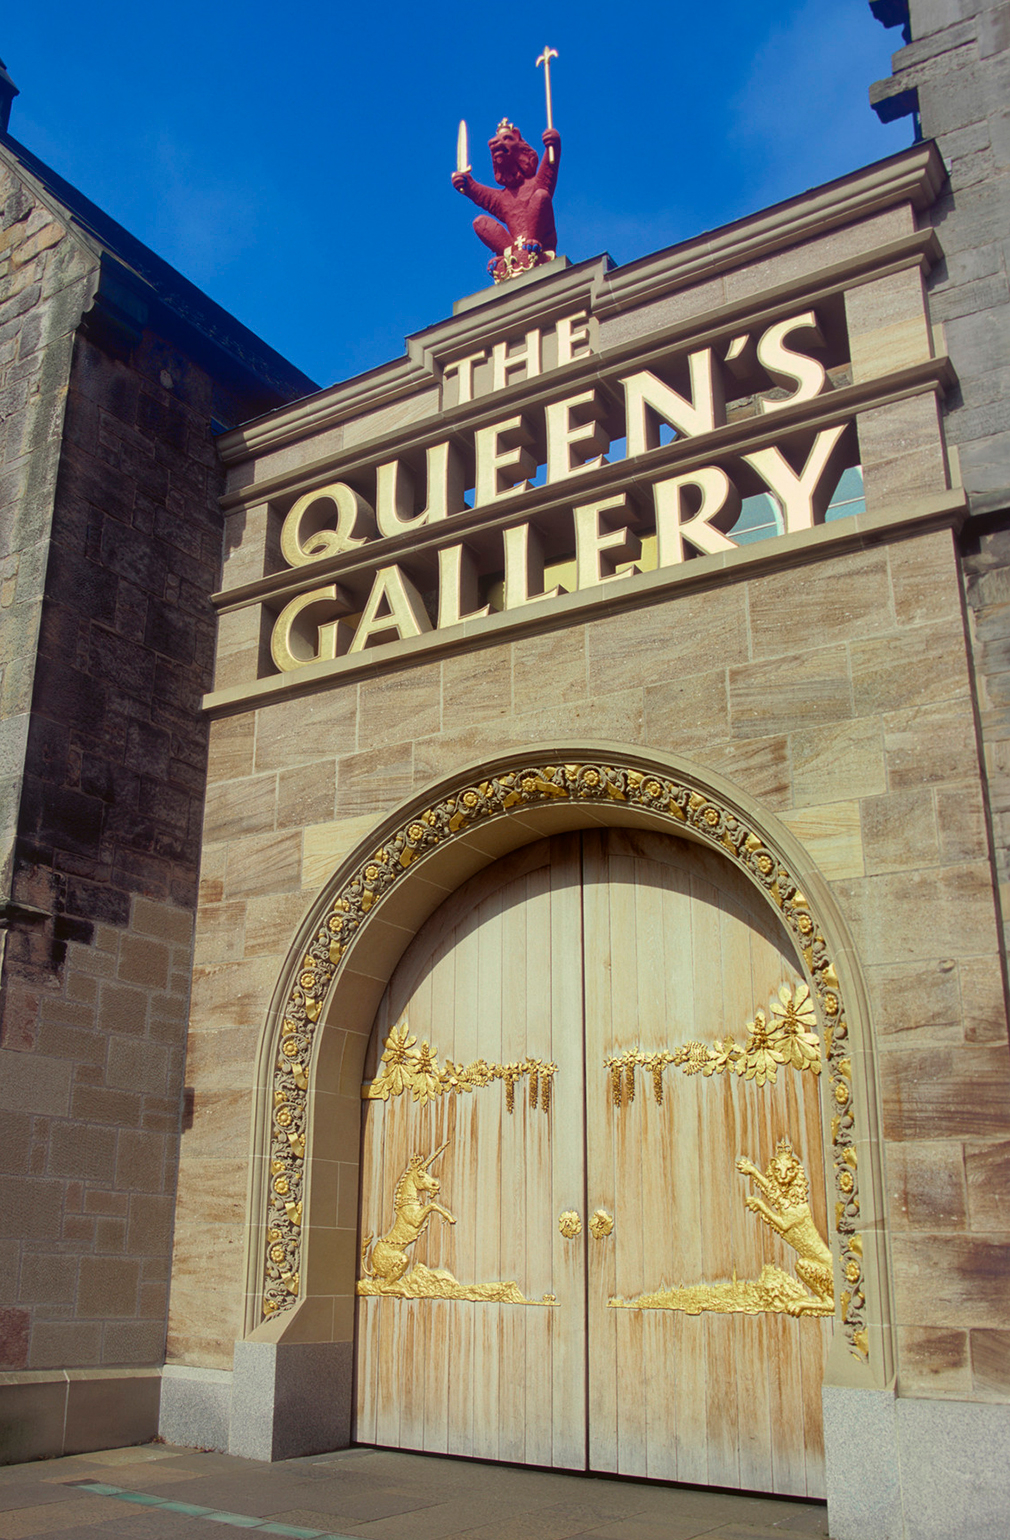
\includegraphics[height=5cm]{figures/gallery-exterior.jpg}
		\caption{Entrance \citep{AboutTheQueensGallery}}\label{fig:qgexterior}
	\end{subfigure}
	\begin{subfigure}[b]{.48\textwidth}
		\centering
		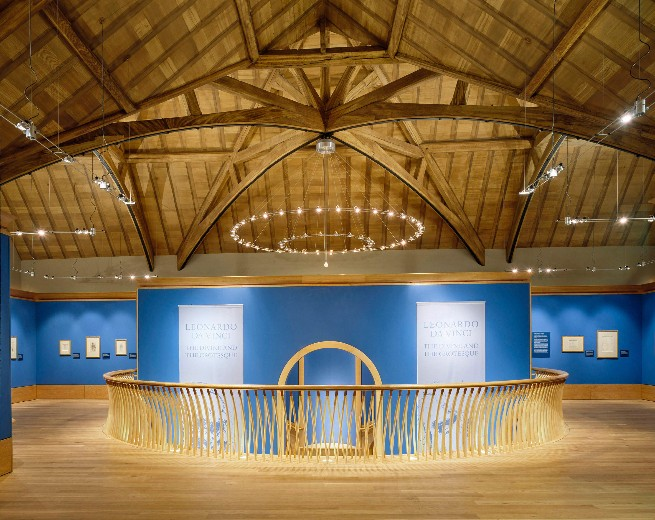
\includegraphics[height=5cm]{figures/gallery-interior.jpg}
		\caption{Interior \citep{InsideTheGallery}}\label{fig:qginterior}
	\end{subfigure}
	\rule{\textwidth}{0.5pt} % use line???
	\caption[The Queen's Gallery and the concept of contextual isolation.]{The Queen's Gallery and the concept of contextual isolation in the design of its building services}
	\label{fig:qg}
\end{figure}





\subsection*{EL3(i, b, m)}

\begin{wraptable}{r}{0.2\textwidth}
	\begin{tabular}{|ll|}
		\hline
		\multicolumn{2}{|c|}{\cellcolor[HTML]{F8A102}\textbf{EL3(i, b, m)}} \\ \hline
		\DST & \LAB \\
		\ICP &  \\ \hline
	\end{tabular}
\end{wraptable}

I gained knowledge of some nascent management techniques that may be used to achieve engineering objectives.
In \ICPTitle, I learned about techniques such as lean construction and supply-chain management (which both have the aim of helping identify flows and wastes) as well as partnering and BIM (which both encourage openness and transparency).

Take lean construction, which is a concept borrowed and adapted from lean manufacturing.
This production method was invented by the Japanese company Toyota shortly after the Second World War.
Japan at the time found itself especially limited in resources due to trade embargoes or restrictions with the Western powers.
Toyota thus had to find a way to make the most use of its restricted resources in order to achieve its production objectives.
Hence, lean manufacturing and construction are about achieving engineering objectives in the most efficient way, i.e. by minimising waste and maximising value.
There are several planning systems that complement this management technique, for example Last Planner which is designed to produce predictable workflows (see Figure~\ref{fig:lastplanner}).


\begin{figure}[htbp]
	\centering
	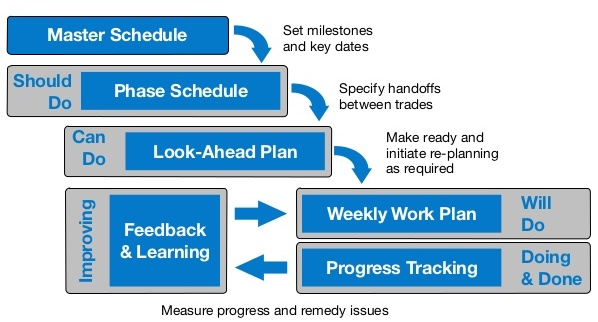
\includegraphics[width=10cm]{figures/last-planner.jpg}
	\rule{10cm}{0.5pt} % use line???
	\caption{The Last Planner system \citep{last-planner}.}
	\label{fig:lastplanner}
\end{figure}


I have some understanding of management techniques since I have used Gantt-like charts on a couple occasions (see Figures~\ref{fig:lab-gantt} and~\ref{DST_schedule}).
When I used the chart to plan the execution of a \LABTitle \space acoustics experiment, it was not very successful.
The chart attempted to coordinate the overlapping activities of our group (which consisted of seven members) within a time limit of 40 minutes so that we could carry out trials on three groups of research participants.
In the end, our experiment ran over time due to our poor timing/ coordination.
The use of the chart was not successful because it was very detailed (on a minute-by-minute basis) and yet we had not familiarised ourselves with it well enough beforehand.
If we were well-rehearsed in the experimental procedure, the use of the Gantt chart could have been more successful.
Hence I learned that there is an element of practice that needs to complement management techniques in order for them to work or run smoothly.

I have not come across change management and do not have enough of experience with management techniques to know their limitations and how they may be applied appropriately.
%Judging from the titles of the upcoming courses of Semester 2, Year 5 (see Table~\ref{tbl:courses}), I suspect I might achieve LO EL3m.
%Considering that this LO should be gained at a Masters level, maybe t
Considering that LO EL3m should be gained at a Masters level, I might learn these things in the second semester of Year 5.
However, judging from the titles of the upcoming courses (see Table~\ref{tbl:courses}), this to me sounds unlikely.





\subsection*{EL4(i, -)}

\begin{wraptable}{r}{0.2\textwidth}
	\begin{tabular}{|ll|}
		\hline
		\multicolumn{2}{|c|}{\cellcolor[HTML]{F8A102}\textbf{EL4(i, -)}} \\ \hline
		\IE & \DPA \\
		\CAS & \EnBldgs \\
		\DI & \FMP \\
		\SIB & \CCSA \\
		\WSD &  \\
		Arup & Hoare Lea \\
		Sunamp & Sweco \\ \hline
	\end{tabular}
\end{wraptable}

I have a good understanding of the requirement for AE activities to promote sustainable development as many of the AE courses have addressed the increasing need for sustainable design to mitigate and adapt to climate change.
%According to the oft-quoted Brundtland report, sustainable development is an approach to progress which meets the needs of the present generation without compromising the ability of future generations to meet their own needs.
%In the context of the built environment, this can be translated as, ``Designing, constructing and managing buildings and resources in such a way that building occupants’ needs are met without the profligate use of energy and resources, such that sufficient provision is left for future generations to provide for themselves" \citep{CCSAunit1}.
%Perhaps because of the direct influence AE has on particularly the energy consumption of a building, many of the courses throughout the programme have addressed the increasing need for sustainable design to mitigate and adapt to climate change.
I especially realised the importance of this engineering requirement as I came across a response CIBSE offered in a governmental consultation during my research for a group poster for \CCSATitle.
%(see description of assignment in \textit{G1} in Section \ref{sec:G1}), 
%At the start of 2018,
Before the publication of the 2018 National Adaptation Programme (NAP) to climate change, 
the government suggested that adaptation reporting continues to be done on a voluntary basis.
However, CIBSE protested by stressing that adaptation is necessary because climate change threats are real and imminent, so reporting should be done on a mandatory basis by even more sectors than have been required of so far \citep{CIBSE:CCAreporting}.
Unfortunately, according to the 2018 NAP, the government will not make reporting mandatory because the majority of the respondents to the consultation favoured the continuation of voluntary reporting \hl{cite NAP from Mendeley}.
Perhaps if more engineering institutions acted like CIBSE and promoted the urgency of sustainable development in this consultation, as is their duty, the government's stance on sustainable development might have been stronger.

\begin{wrapfigure}{r}{0.5\textwidth}
	\centering
	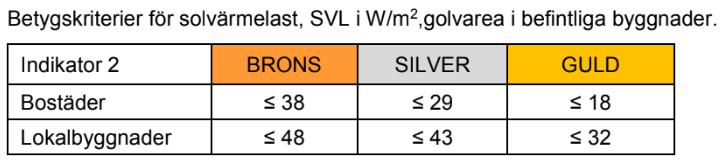
\includegraphics[width=0.5\textwidth]{figures/SVL.PNG}
	\rule{0.5\textwidth}{0.5pt} % use line???
	\caption[The \textit{Miljöbyggnad} assessment criteria for solar heat gains in existing buildings.]{The \textit{Miljöbyggnad} assessment criteria for solar heat gains (in W/m\textsuperscript{2}) in existing buildings \hl{cite miljobyggnad}.}
	\label{fig:svl}
\end{wrapfigure}

I also have the ability to apply quantitative techniques to promote sustainable development.
An example is the work I did at Sweco on environmental certification, a way to promote the sustainable design of buildings.
I calculated and ranked things like solar heat gains, energy consumption and daylighting according to \textit{Miljöbyggnad}'s standards of what qualified as a sustainable building (see Figure~\ref{fig:svl}).


%According to the oft-quoted Brundtland report, sustainable development is an approach to progress which meets the needs of the present generation without compromising the ability of future generations to meet their own needs.
%\hl{Can't think of examples. Also, ability to apply quantitative techniques???}



\subsection*{EL5(-, m)}

The following courses increased my awareness of legal requirements governing engineering activities including \hl{health and safety (H\&S)}, liability issues, contracts and accessibility:
\textit{Design Issues},
\textit{Procurement and Contracts},
and \textit{Inclusive and Safe Environments}.
In particular, in \textit{Design Issues} I learned about the various UK regulations surrounding H\&S, including the Health and Safety at Work Act 1974 and the Construction (Design and Management) Regulations 2015, a.k.a. the CDM Regulations.
The CDM Regulations emphasise that H\&S need to be considered, not just on site, but throughout the planning and design stages also.
The designers, for example, have a responsibility to assess and eliminate or mitigate the H\&S risks associated with their design, whether that is during the construction or operation of the building.
Furthermore, this course broadened my awareness of legal requirements outside of the UK.
I learned about the H\&S regulations in France, the lack of building regulations in Guyana, and the ambitious building regulations with regards to sustainability in Singapore.
\hl{Is that a good demonstration of my knowledge? David: provide two references.}

I have also applied my knowledge of legal requirements in a project for \textit{Inclusive and Safe Environments} and during my placements at Hoare Lea and Sweco.
At Hoare Lea I produced \hl{RIBA} Stage 3 layouts of fire detection and alarm installations for a new-build.
These were made to comply with standards such as \textit{BS 5839-6:2013 Fire detection and fire alarm systems for buildings - Part 6: Code of practice for the design, installation, commissioning and maintenance of fire detection and fire alarm systems in domestic premises}.
For instance, the standard stated the different radiuses that smoke detectors and heat detectors cover; I had to thus place the detectors on the plan layouts accordingly.


\subsection*{EL6(i, b, m)}

Many courses and a couple of my placements increased my awareness of risk issues.
I learned about risk issues related to H\&S at Sunamp and in
\textit{Electrical and Lighting Services for Buildings},
\textit{Design Issues},
\textit{Inclusive and Safe Environments},
and
\textit{Laboratory Project}.
In \textit{Electrical and Lighting Services for Buildings}, for example, I learned about the importance of earthing to give \hl{overflow?} electricity an alternative path to run through which is not a person (thus electrocuting them).
I learned about environmental risk issues in
\textit{Construction Technology 1},
\textit{Introduction to the Environment},
\textit{Thermal Performance Studies},
\textit{Sustainable and Intelligent Buildings},
\textit{Climate Change, Sustainability and Adaptation},
and
\textit{Water Supply and Drainage for Buildings}.
Throughout these courses I have learned about the impact of buildings and building systems on the environment, e.g. harmful refrigerants in air conditioners, embodied carbon in building materials, and the emissions from vehicles that people use to travel to buildings.
Lastly, I learned about \hl{commercial risk (?)} in \textit{Innovation in Construction Practice}, more specifically the risk of innovation in construction projects.
\hl{Elaborate?}

I learned about the techniques of risk assessment and risk management in depth in \textit{Design Issues} and have carried out H\&S risk assessments in \textit{Facilities Management Principles}, \textit{Laboratory Project} and during my placement at Arup.
\hl{Attach LAB risk assessments?}
Generally, one first needs to identify the risks and then assess them in terms of severity and likelihood.
Afterwards, one tries to eliminate the risks (the worst first), and if that is not possible, mitigate them.


\subsection*{EL7m}

For business success, I have only gained an understanding of how innovation is a key driver in \textit{Innovation in Construction Practice} and \hl{how technology (?) plays a role in business success through the study of Fordist and post-Fordist consumerism/ manufacturing?} in \textit{Sustainable and Intelligent Buildings}.
\hl{Look up ICP and SIB notes + elaborate.}

Due to the nature of my academic programme, I have not learned as much about the key drivers for business success as I have for successful construction projects in the following courses:
\textit{Introduction to Design},
\textit{Procurement and Contracts},
\textit{Facilities Management Principles},
\hl{and more?}
However, there are two ways that this knowledge can translate to business.
Firstly, a construction project is often a means for a business to grow or improve (\hl{this is known as a secondary business case? see FM notes}).
Therefore, a successful construction project can lead to a successful business.
Secondly, the principles behind a successful construction project should also be able to be applied to businesses.
For example, after the construction sector was pointed out in the 1990s for repeatedly delivering projects that were of poor quality, overtime and over-budget, the sector has made significant efforts to improve its performance and improve client satisfaction.
Such efforts have resulted in changing the workflow so that more planning is done at the start of a project, when making changes is more flexible and less costly (\hl{get figure from ICP?}).
This includes developing more descriptive briefs, which set out the client's needs and how the construction project should be run.
\hl{I imagine this could translate in such a way to business... think!}



%----------------------------------------------------------------------------------------
%	SECTION 5
%----------------------------------------------------------------------------------------
\newpage
\section{Engineering Practice (P)}


\subsection*{P1(i, -)}

\begin{wraptable}[10]{r}{0.2\textwidth}
    \begin{tabular}{|ll|}
        \hline
        \multicolumn{2}{|c|}{\cellcolor[HTML]{F8A102}\textbf{P1(i, -)} \nomaster} \\ \hline
        \BST & \IE \\
        \DPA & \Acoustics \\
        \EnvBeh & \EPA \\
        \DPB & \CAS \\
        \ELS & \EnBldgs \\
        \TPS & \DI \\
        \FMP & \PRJ \\
        \DST & \LAB \\
        \SIB & \CCSA \\
        \WSD &  \\
        Arup & Hoare Lea \\
        Sunamp & Sweco \\ \hline
    \end{tabular}
\end{wraptable}

Throughout the programme, I have gained knowledge and understanding of some contexts in which my AE knowledge can be applied.
The following list, in which I describe such contexts, is not exhaustive.

\begin{enumerate}
	\item %The collaborative design projects in years \hl{1/2} and 4,
	%\textit{Building Services Technology},
	%\textit{Introduction to the Environment},
	%\textit{Design Project A},
	%\textit{Design Project B},
	%\textit{Electrical and Lighting Services for Buildings},
	%\textit{Critical Architectural Studies},
	%\textit{Design Project},  
	Several courses throughout the years and my placements at Arup and Hoare Lea
	provided me with the practical experience of applying my AE knowledge in the context of a team designing a building and/ or its services, in which I was responsible for the building services, the building's internal environment and the occupants' comfort levels.
	My group's first prize for sustainability (see Figure~\ref{fig_award}) demonstrates my understanding of an Architectural Engineer's role in passive design (e.g. natural lighting).
	
	\item Throughout several courses (especially \FMPTitle),
	%\textit{Acoustics and Architectural Design},
	%\textit{Environment and Behaviour},
	%\textit{Energy Principles and Applications},
	%\textit{Energy and Buildings},
	%\textit{Thermal Performance Studies},
	%\textit{Design Issues},
	%\textit{Facilities Management Principles},
	%\textit{Laboratory Project},
	%\textit{Sustainable and Intelligent Buildings},
	%\textit{Climate Change, Sustainability and Adaptation},
	%\textit{Water Supply and Drainage for Buildings},
	my work in the environmental certification of existing buildings at Sweco,
	and
	my encounter with a specialist in Performance at Hoare Lea,
	%Design Issues,
	I have also learned that my AE knowledge is applicable in the operation and management of buildings and building services (a.k.a. facilities management) to, for example, improve the occupants' comfort levels, optimise performance or increase resilience to future impacts of climate change.
	
	\item Through the work I did at Sunamp as well as my encounter with a technical author at Hoare Lea, I understand that engineering knowledge is important in the composition of technical documents (e.g. specifications, operation and maintenance manuals) and even marketing material for technical products, which may need to explain engineering processes graphically and in layman's terms.
	See how I did this in the UniQ PISs in Appendix~\ref{App:PISs}.
	
	\item My dissertation in particular taught me that engineering knowledge is necessary for the development of industry standards and codes of practice, such as the series of Publicly Available Specifications (PAS) 1192 which standardise the requirements for achieving BIM Level 2.
	
	\item Throughout my dissertation and \textit{Climate Change, Sustainability and Adaptation} (\CCSA), I have also come to understand that my engineering knowledge can be used for research, the development of new technologies or processes, and to influence policies.
	One of the assignments for \CCSA \space was to write a briefing for politicians;
	mine urged them to develop policies to make the existing UK housing stock resilient to future climate impacts.
	%\hl{Repeated DST and CCSA. Could even include Sunamp. Maybe this example is one too many...}
\end{enumerate}




\subsection*{P2(i, b, m)}

\begin{wraptable}[12]{r}{0.2\textwidth}
    \begin{tabular}{|ll|}
        \hline
        \multicolumn{2}{|c|}{\cellcolor[HTML]{F8A102}\textbf{P2(i, b, m)} \nomaster} \\ \hline
        \ConTechOne & \BST \\
        \DPA & \ConTechTwo \\
        \Acoustics & \EnvBeh \\
        \Stats & \DPB \\
        \CAS & \ELS \\
        \DSA & \EnBldgs \\
        \TPS & \PRJ \\
        \DST & \LAB \\
        \SIB & \ICP \\
        H\&L & Arup \\
        Hoare Lea & Sunamp \\ \hline
    \end{tabular}
\end{wraptable}

I have gained knowledge of the characteristics of, an understanding of and an ability to use a range of computer-based tools, engineering processes, and building services products:
\begin{itemize}
    %\item P2i 
     
    % In \textit{Environment and Behaviour}, \textit{Laboratory Project} and \textit{Dissertation}, I developed an ability to use the statistics software tool SPSS (Statistical Package for the Social Science).
    % The course \textit{Statistics for Science} provided me with a foundation to understand the data in the inputs and outputs of this software.
    
    \item \textbf{P2i and P2b}
    
    In \textit{Design Software Applications} and \textit{Laboratory Project}, I gained knowledge of the characteristics of steady-state and dynamic building modelling and energy analysis software programmes, notably iSBEM, SAP, IES, and CFD [\textbf{P2b}].
    As these courses only provided an introduction to these software programmes, I have not mastered my ability to use them [\textbf{P2i}].
    %\hl{Look up} \DSATitle \space \hl{notes if you want to demonstrate knowledge.}
    This was demonstrated during my attempt to model my \textit{Design Project} building in IES; my building model overheated due to variation and temperature profiles that I had incorrectly set up, amongst other things.
    
    %During the \textit{Design Project} and my placements at Hultin \& Lundquist Arkitekter and Sunamp, I gained an understanding of and an ability to use Autocad.
    %Likewise, I learned to use Revit during the \textit{Design Project} and my placements at Arup and Hoare Lea.
    %Although my ability to use these Autodesk products (i.e. Autocad and Revit) is limited, I have learned quite a bit about their characteristics.
    %In \textit{Dissertation} and \textit{Innovation in Construction Practice}, I learned about the prominent use of these products in the UK construction industry and how their proprietary characteristics can lead to problems of interoperability.
    
    Regarding engineering processes, 
    %I have learned extensively about the BIM process in Dissertation and Innovation in Construction Practice.
    I have learned the characteristics of and practised the optimisation process of an engineering design in \textit{Laboratory Project} (see \textit{EA3(i, b, m)} in Section \ref{EA3} for more detail) [\textbf{P2i and P2b}].
    
    \item \textbf{P2m}
    
    Throughout many of my construction-based courses and my placements at Sunamp, Hoare Lea and Arup,
    I have accumulated an extensive knowledge of a wide range of building services products (e.g. heat pumps, heat batteries, PV panels) and building materials (e.g. PCMs, Ziegel blocks, steel).
    My understanding of these products and materials, however, varies.
    %\hl{Elaborate with heat pump drawing and compare with Ziegel blocks, for example.}
    %throughout many of my construction-based courses, i.e. 
    %\textit{Construction Technology 1},
    %\textit{Building Services Technology},
    %\textit{Design Project A},
    %\textit{Construction Technology 2},
    %\textit{Acoustics and Architectural Design},
    %\textit{Design Project B},
    %\textit{Critical Architectural Studies},
    %\textit{Electrical and Lighting Services for Buildings},
    %\textit{Design Software Applications},
    %\textit{Energy and Buildings},
    %\textit{Thermal Performance Studies},
    %\textit{Design Project},
    %\textit{Laboratory Project},
    %\textit{Sustainable and Intelligent Buildings},
    %\textit{Innovation in Construction Practice},
    %and \textit{Water Supply and Drainage for Buildings},
    %and my placements at Sunamp, Hoare Lea and Arup
\end{itemize}

\begin{comment}
	\begin{wrapfigure}{r}{0.3\textwidth}
	\centering
	\begin{subfigure}{0.3\textwidth}
	\centering
	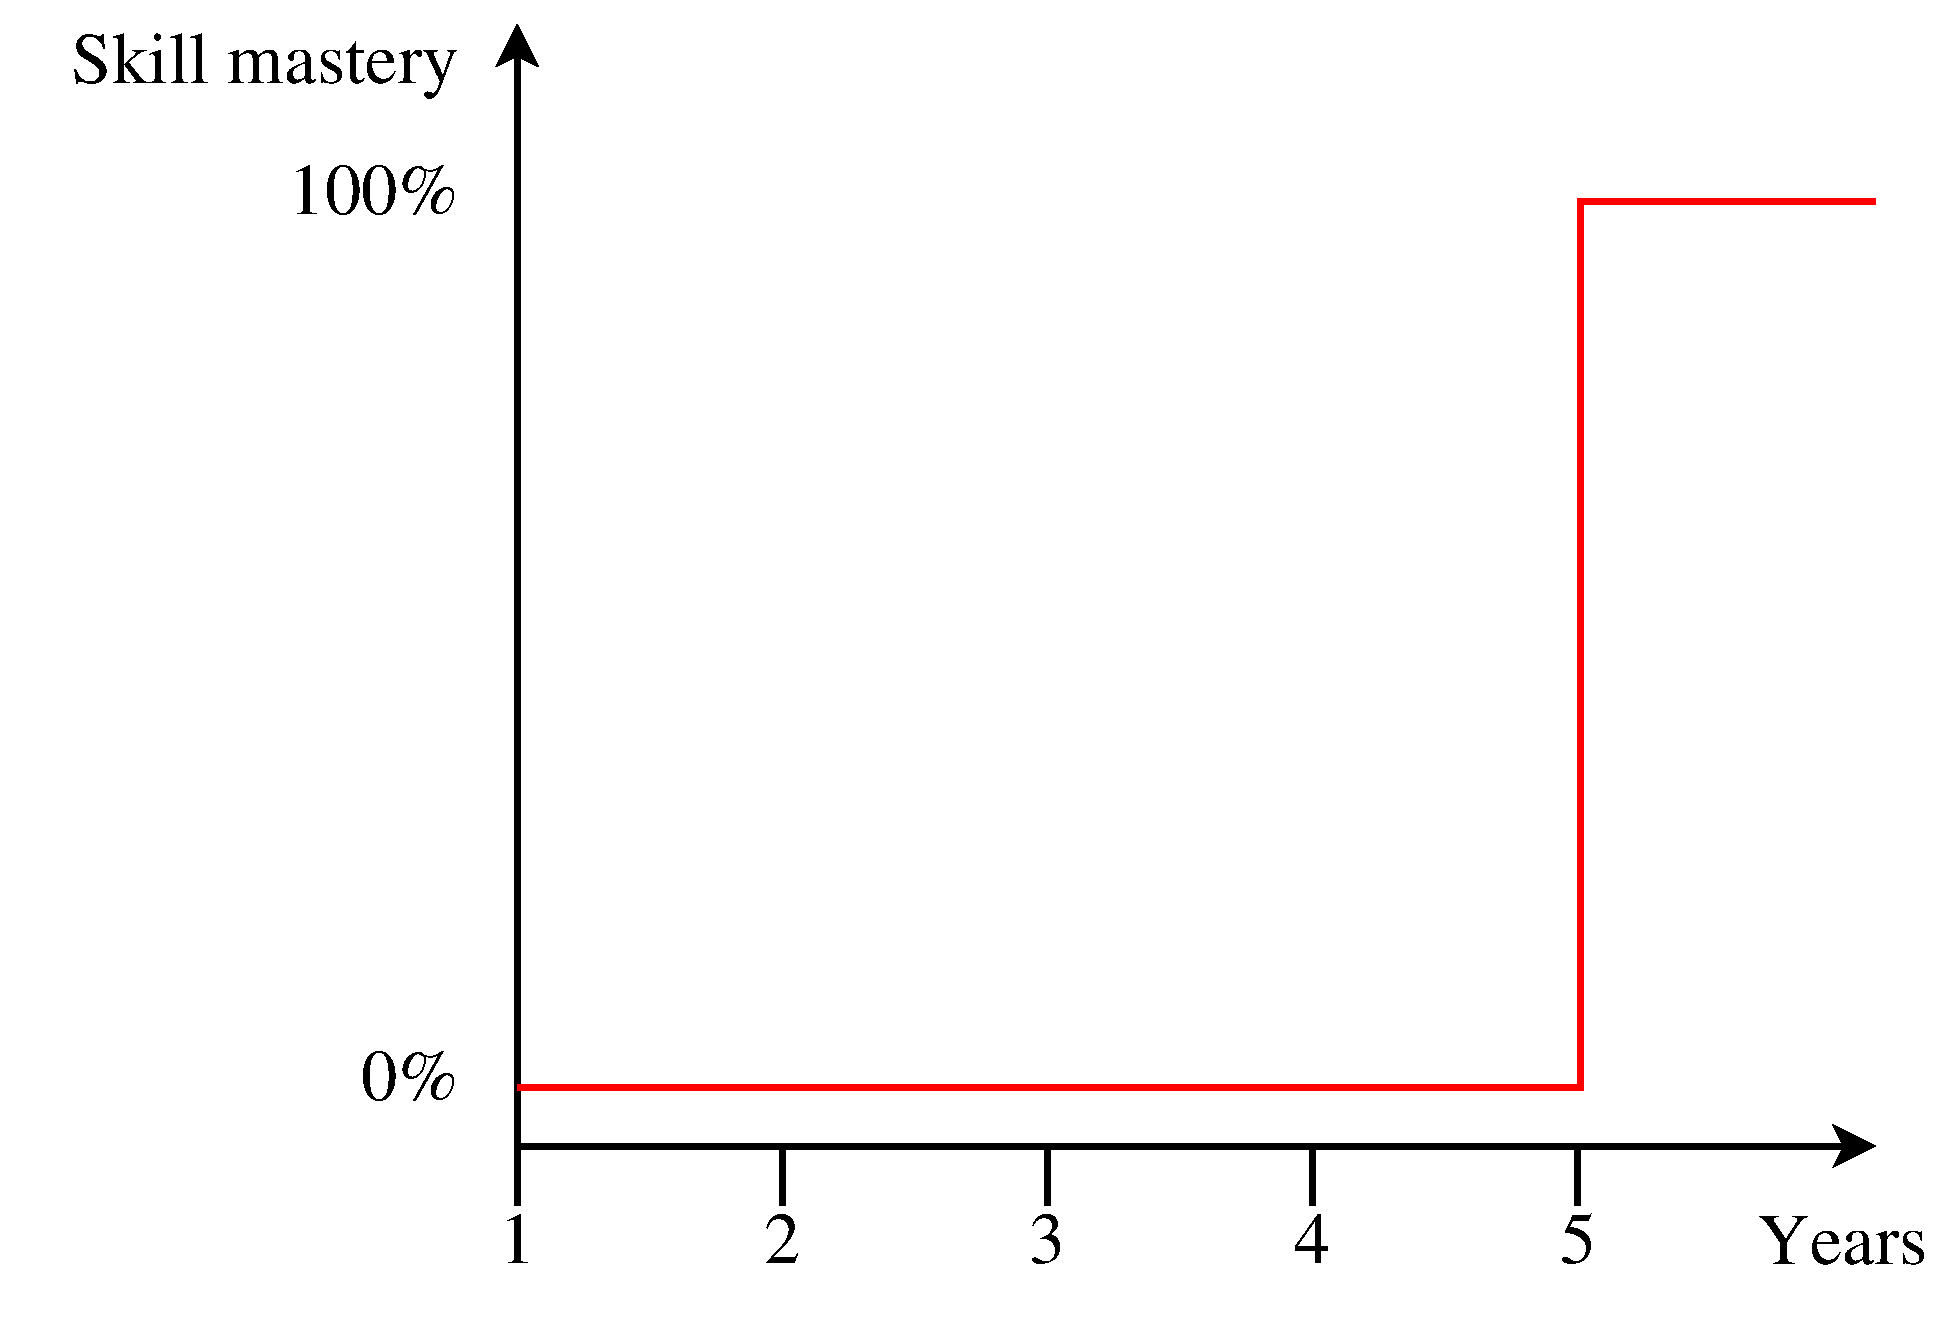
\includegraphics[width=\textwidth]{figures/learning-zigzag.eps}
	%          \rule{\textwidth}{0.5pt} % use line???
	\caption{Unrealistic}
	\label{}
	\end{subfigure}
	\begin{subfigure}{0.3\textwidth}
	\centering
	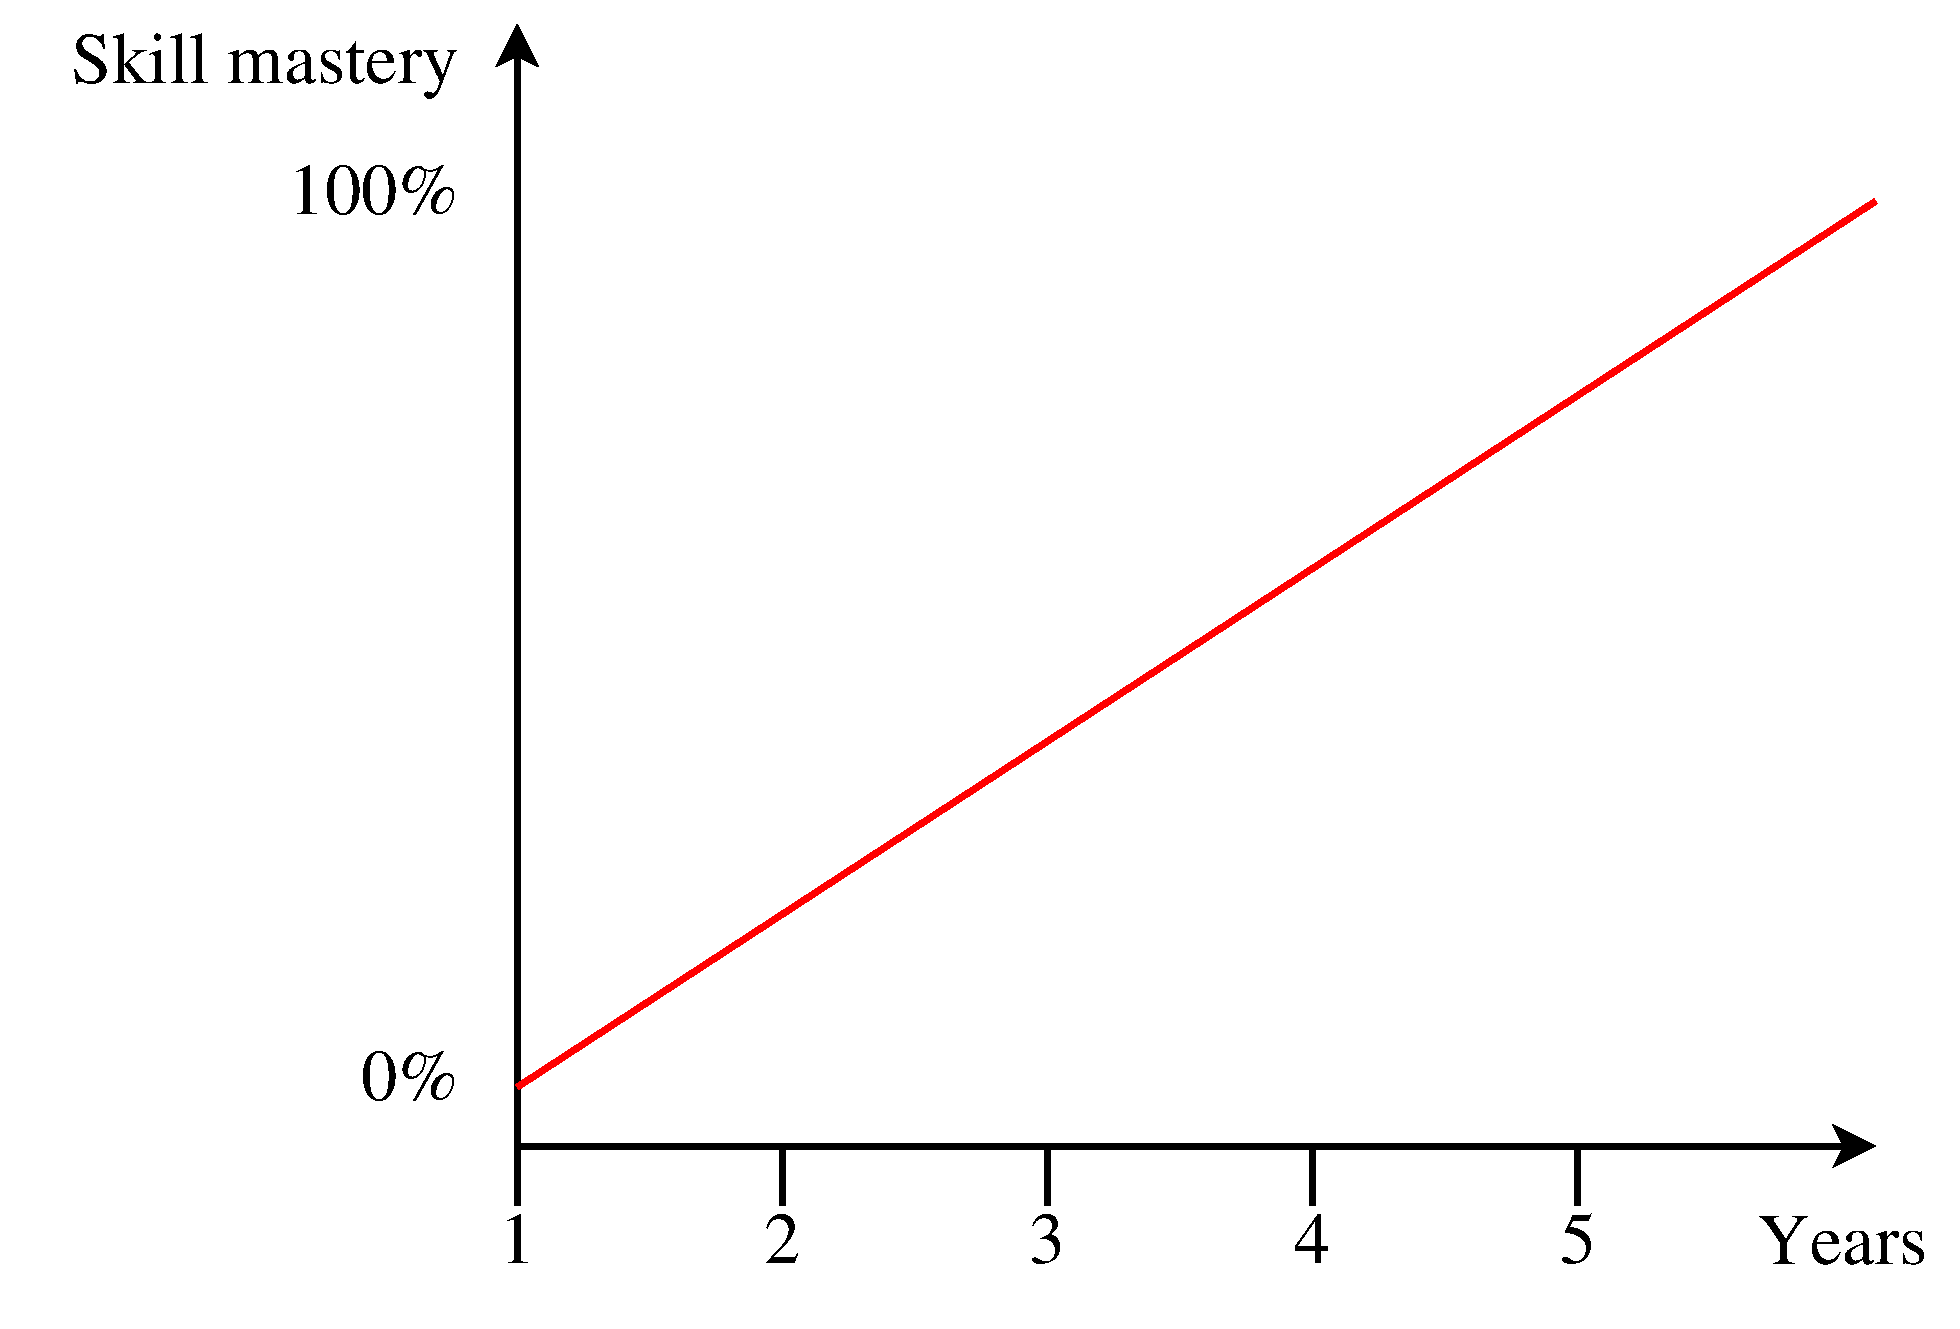
\includegraphics[width=\textwidth]{figures/learning-curve.eps}
	%          \rule{\textwidth}{0.5pt} % use line???
	\caption{Incremental}
	\label{}
	\end{subfigure}
	\rule{0.3\textwidth}{0.5pt} % use line???
	\caption{Ways to gain knowledge and understanding.}
	\label{}
	\end{wrapfigure}
\end{comment}



%\hl{Move following explanation to chapter intro?}
N.B. P2m is a LO for Masters students.
However, I do not think it is reasonable to assume that somebody can gain an extensive knowledge and understanding of a wide range of engineering materials and components (or most of anything) exclusively at Masters level, as shown in Figure~\ref{fig:learning01}.
I believe this is a cumulative process as shown in Figure~\ref{fig:learning02}, which is why, in my skills matrix, I have marked courses since Year 1 as having contributed to my attainment of this LO.


\begin{figure}[htbp]
	\centering
	\begin{subfigure}{.48\textwidth}
		\centering
		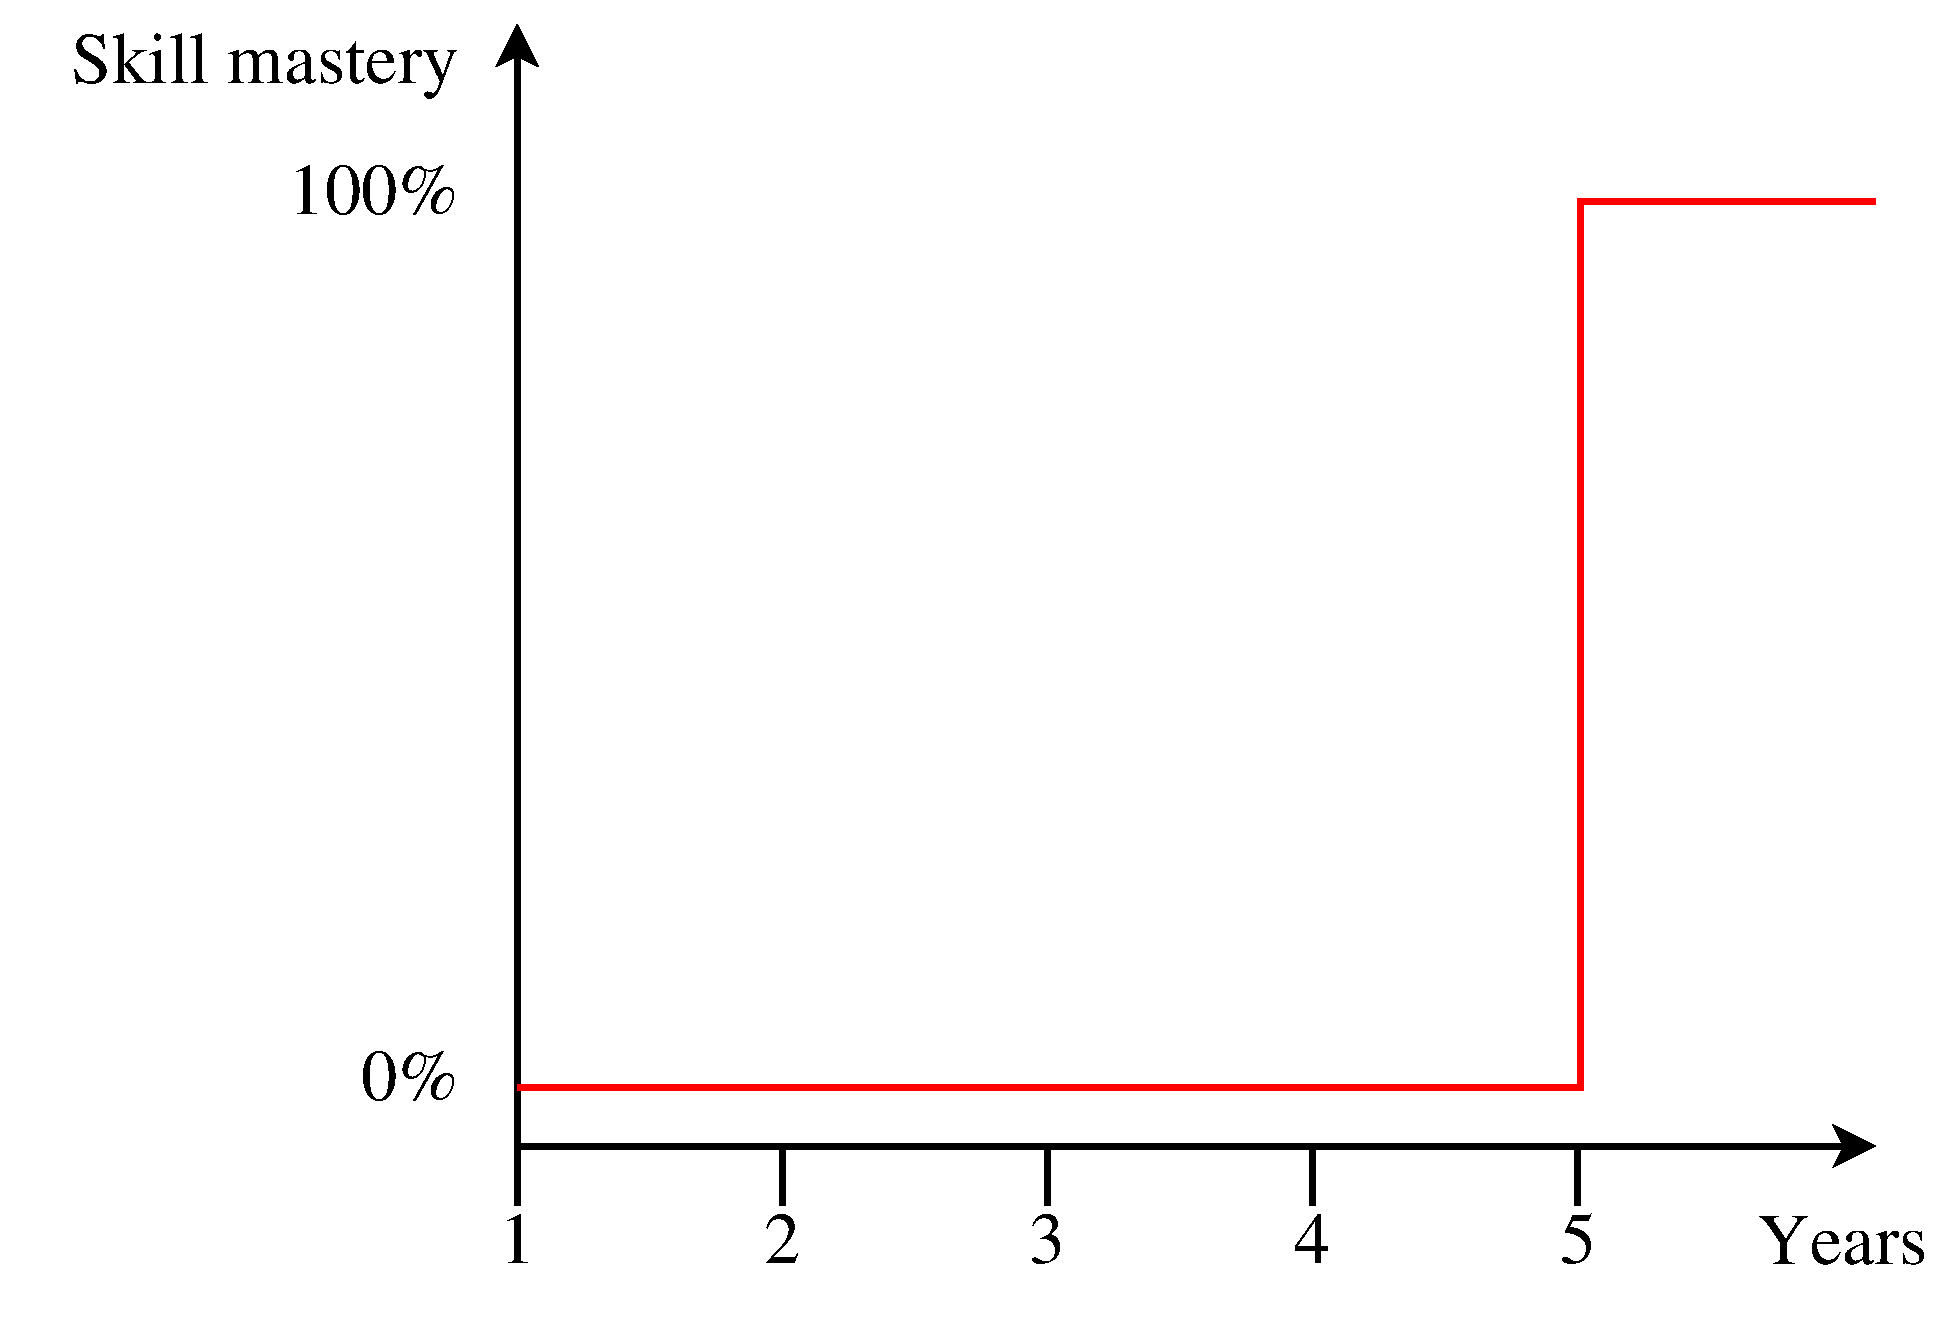
\includegraphics[width=0.75\textwidth]{figures/learning-zigzag.eps}
		%          \rule{\textwidth}{0.5pt} % use line???
		\caption{Unrealistic}
		\label{fig:learning01}
	\end{subfigure}
	\begin{subfigure}{.48\textwidth}
		\centering
		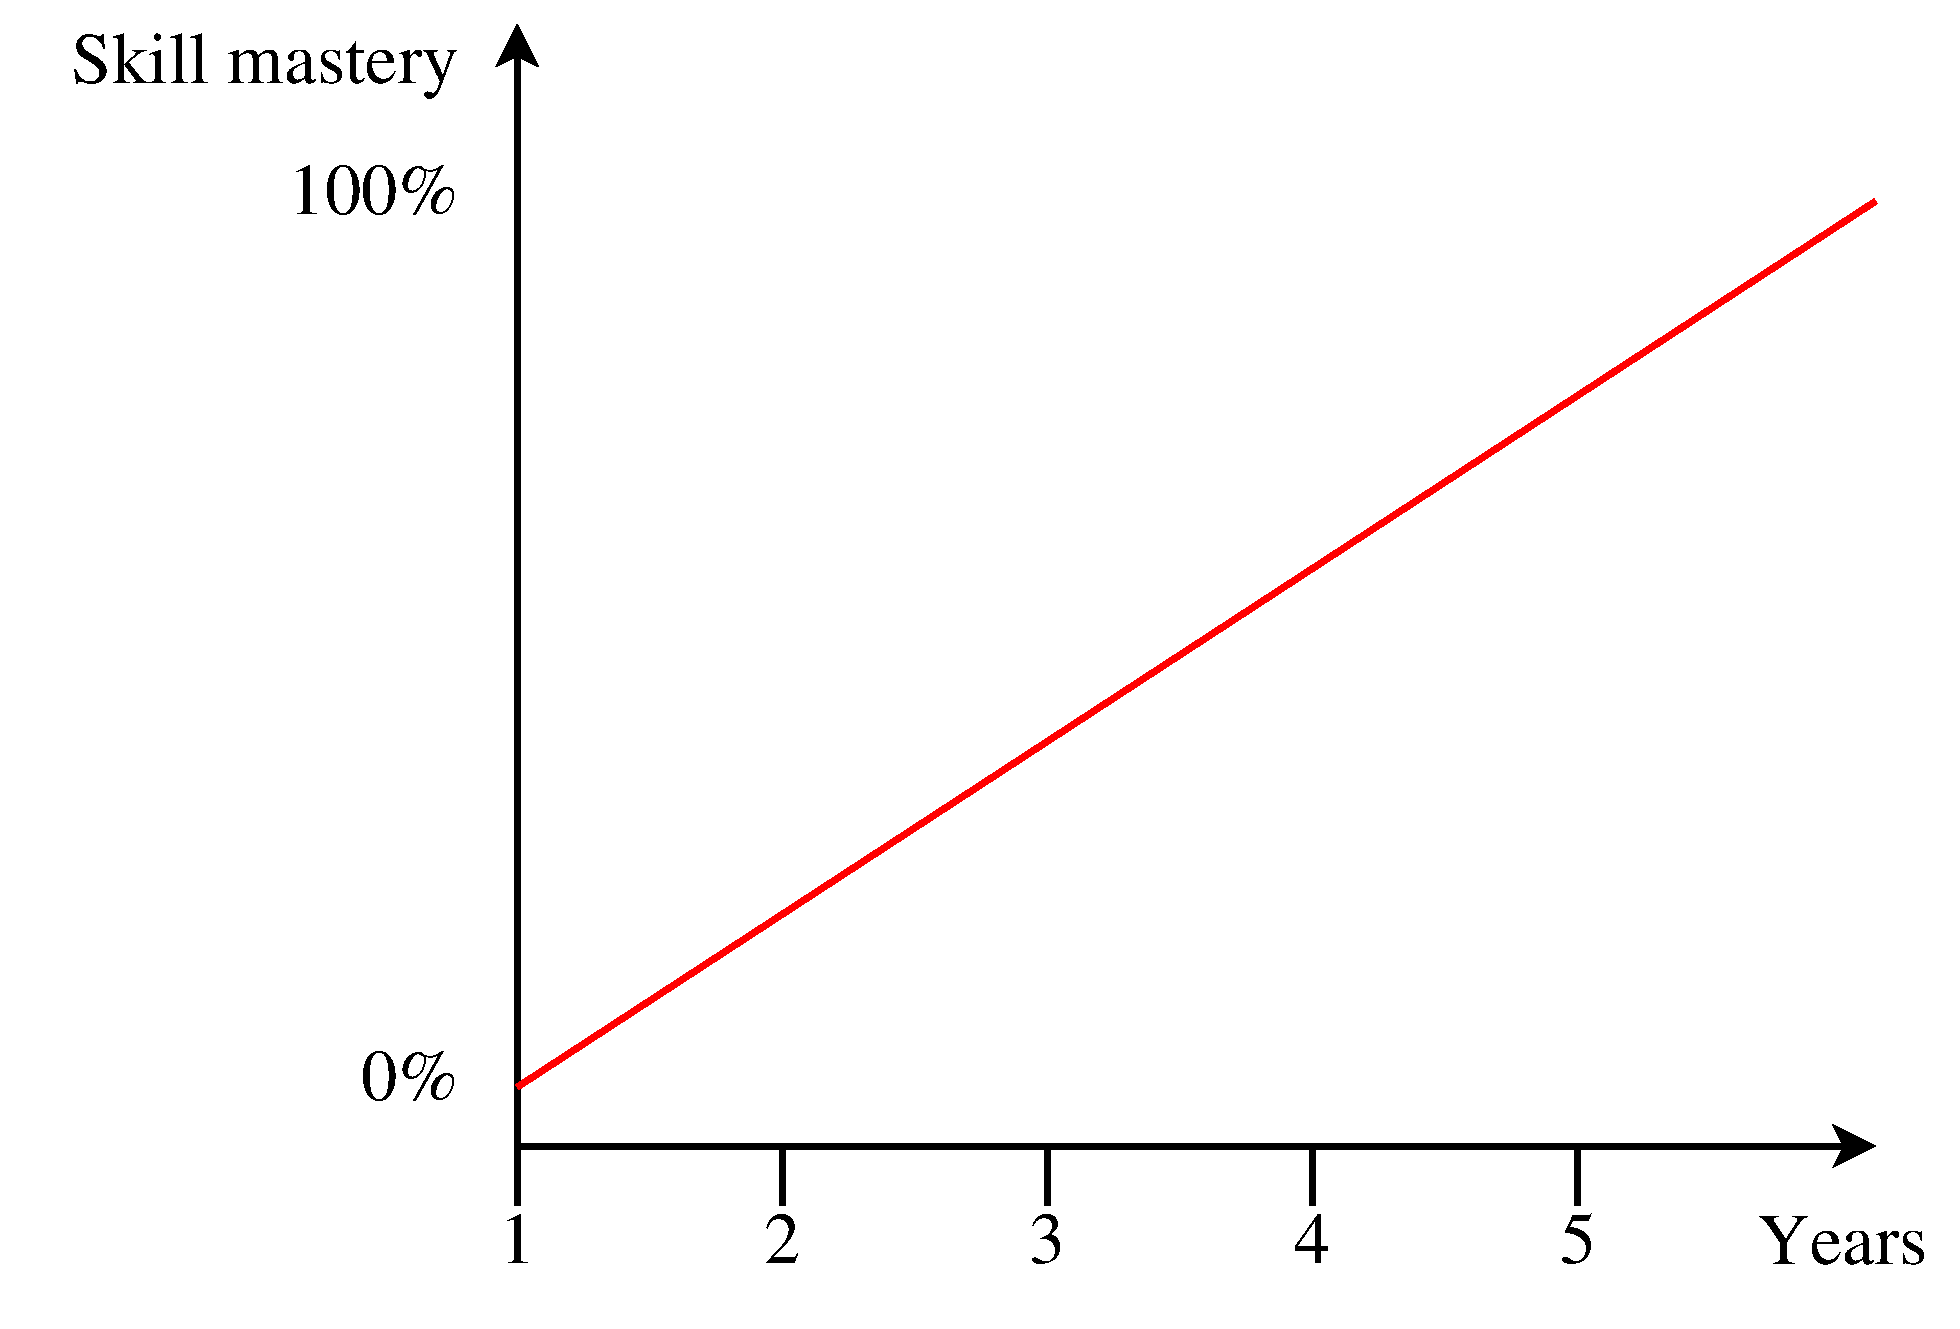
\includegraphics[width=0.75\textwidth]{figures/learning-curve.eps}
		%          \rule{\textwidth}{0.5pt} % use line???
		\caption{Incremental}
		\label{fig:learning02}
	\end{subfigure}
	\rule{\textwidth}{0.5pt} % use line???
	\caption{Ways to gain knowledge and understanding.}
	\label{fig:learning}
\end{figure}


%\hl{Write about increase in knowledge throughout the years. P2m for example couldn't all of a sudden have been achieved in Y5.}

%Building materials: insulation, steel, wood, Ziegel blocks, glass, PCMs etc.

%Building services products: ACs, HPs, PV, AHUs, Sunamp, windcatchers




\subsection*{P3(i, -)}

\begin{wraptable}{r}{0.2\textwidth}
    \begin{tabular}{|ll|}
        \hline
        \multicolumn{2}{|c|}{\cellcolor[HTML]{F8A102}\textbf{P3(i, -)} \master} \\ \hline
        \ConTechTwo & \Acoustics \\
        \HYD & \EPA \\
        \CAS & \TPS \\
        \LAB &  \\ \hline
    \end{tabular}
\end{wraptable}

%\begin{itemize}
%    \item \textbf{P3i}
    
    I have already had laboratory practice in physics, chemistry and biology in high school.
    In university, my knowledge and understanding of laboratory practice began to further develop in Year 2 when I conducted experiments in \textit{Construction Technology 2}, \textit{Acoustics and Architectural Design}, \textit{Hydraulics and Hydrology A} and \textit{Energy Principles and Applications} [\textbf{P3i}].
    The feedback for my hydraulics lab report of 93\% demonstrates my knowledge and understanding of laboratory practice.
    
%    \item \textbf{P3}
    
    In Years 3 and 4, I gained the ability to apply practical and laboratory skills that were more relevant to AE through my increased exposure to and application of laboratory practice in thermofluids and acoustics [\textbf{P3}].
    I re-visited the Services lab another two times for thermofluids-related experiments in \textit{Thermal Performance Studies} and \textit{Laboratory Project} and re-used my practical skills of recording, measuring and analysing sounds in \textit{Critical Architectural Studies} and \textit{Laboratory Project}.
%\end{itemize}

My final mark of 73\% in the \LABTitle \space demonstrates my full achievement of LOs P3i and P3.
%\hl{What actions and results can I show as evidence of my practical skills?}



\newpage
\subsection*{P4(i, -)}

\begin{wraptable}{r}{0.2\textwidth}
    \begin{tabular}{|l|}
        \hline
        \rowcolor[HTML]{F8A102} 
        \multicolumn{1}{|c|}{\cellcolor[HTML]{F8A102}\textbf{P4(i, -)} \littlemaster} \\ \hline
        \PRJ \\
        Sunamp \\ \hline
    \end{tabular}
\end{wraptable}

I have developed the ability to use and apply information from technical literature during my \PRJTitle \space and my Sunamp placement [\textbf{P4i}].
For the \PRJTitle, I sought, used and applied information from product specifications in order to size my building's water storage tank \citep{Decca}, calorifiers and buffer vessels \citep{RycroftLtd} etc.
At Sunamp, I used their technical manuals in order to produce the UniQ PISs (Appendix~\ref{App:PISs}).
%The technical literature I have been exposed to includes Sunamp's manuals for their UniQ product range and the product information sheets I drew up for them.
These sheets included information such as temperature input and output ranges, schematic diagrams, and the dimensions of the heat batteries.
%\hl{Include evidence, e.g. attach PISs}

%I also came across and used technical literature during my \textit{Design Project}.
%I used product specifications to size the college's water storage tank \citep{Decca}, calorifiers and buffer vessels \citep{RycroftLtd} etc.

Throughout my \textit{Design Project} and Sunamp experiences, I gained an understanding of the use of technical literature [\textbf{P4}].
%During the Design Project, I used technical literature to appropriately size some of the building services, both to accommodate the needs of the building's occupants and to fit inside of the plant room.
For example, at Sunamp, I was part of the decision-making process of the information that should be included in the UniQ PISs, which would be one of the first documents a customer would see once they have taken interest in Sunamp's products.
It was decided that information such as dimensions and weight were important to include for a couple reasons.
Firstly, to highlight the compact size of Sunamp's batteries (which is one of their unique selling points).
Secondly, to give the customers an indication of the transportation and placement requirements of a battery (e.g. depending on the type and size, a single UniQ battery will weigh between 55 kg and 211 kg 
%be it may need to be carried by two people and 
and will thus need to be placed on a load-bearing floor).
%\hl{Perhaps do not be afraid to write more sentences and give details such as specific weights and dimensions, and talk about stacking batteries and load bearing floors vs shelves etc.}


\subsection*{P5}

\begin{wraptable}{r}{0.2\textwidth}
	\begin{tabular}{|l|}
		\hline
		\rowcolor[HTML]{F8A102} 
		\multicolumn{1}{|c|}{\cellcolor[HTML]{F8A102}\textbf{P5} \littlemaster} \\ \hline
		\PC \\
		\DI \\ \hline
	\end{tabular}
\end{wraptable}

Considering that in the UK-SPEC defines knowledge as information that can be recalled, I do not have much knowledge of legal and contractual issues relevant to AE.
We have, however, covered contracts in \textit{Procurement and Contracts} and professional liability and insurance in \textit{Design Issues}.
It is perhaps due to a lack of coursework or examination and/ or a lack of spaced repetition of these topics throughout my degree programme that have I not gained a firm knowledge in relevant legal and contractual issues.





\subsection*{P6(i, -)}

\begin{wraptable}[5]{r}{0.2\textwidth}
	\begin{tabular}{|ll|}
		\hline
		\multicolumn{2}{|c|}{\cellcolor[HTML]{F8A102}\textbf{P6(i, -) \littlemaster}} \\ \hline
		\PRJ & \DST \\
		\ISE & H\&L \\
		Hoare Lea & Sweco \\ \hline
	\end{tabular}
\end{wraptable}

I have used appropriate codes of practice and industry standards during \textit{Design Project}, \textit{Inclusive and Safe Environments} and my placements at Hoare Lea and Sweco.
For the \textit{Design Project}, for example, I wanted to use water source heat pumps (WSHPs) to generate heat for the college I was designing since it was located right next to a body of water (see Figure \ref{fig:revit}).
I had to figure out how WSHPs could fit into the building's heating strategy.
To do this, I read about WHSPs in CIBSE CP2, the UK's Code of Practice for surface WSHPs.
I decided, because the college was a large non-domestic facility, to use a multi-valent heating system, where the WSHPs would provide the base heating load and some micro combined heat and power (CHP) units would satisfy the peak heating demands \citep[pp.~12,~38]{CP22016}.
%\hl{I have no feedback to demonstrate this specifically was good and my grade for DP wasn't good because of missing elements...}

I do not have a full understanding of appropriate codes of practice and industry standards as I have not had enough exposure to these.
My dissertation, however, has familiarised me with the UK BIM standards (particularly PAS 1192-2) quite well.
I believe my understanding will develop further once I start working in industry, as many of my building consultancy-type placements so far have required me to refer to such documents.






\subsection*{P7}

\begin{wraptable}{r}{0.2\textwidth}
    \begin{tabular}{|ll|}
        \hline
        \multicolumn{2}{|c|}{\cellcolor[HTML]{F8A102}\textbf{P7} \master} \\ \hline
        \EnvBeh & \CAS \\
        \FMP & \LAB \\
        \ICP & Sweco \\ \hline
    \end{tabular}
\end{wraptable}

I have gained an awareness of quality issues and their application to continuous improvement.
Regarding building services, perhaps the most pertinent example is the use of POEs.
POEs are useful ways to collect both objective and subjective data about the operation of a building, the purpose of which is to feed forward into the improvement of that and other buildings' performance.
For the design competition in \CASTitle, I took the initiative to create a POE in the form of a questionnaire which my group used to collect subjective data on the user and staff experiences of the Newington and Wester Hailes libraries in Edinburgh.
We used this data in our improved re-design of Newington Library to redress the problems that had been addressed.
For example, the old library fenestration design failed to exclude sunlight, which caused glare on computer monitors amongst other things.
Therefore, in my lighting and window design, I analysed the sun path and used frosted glazing on south-facing fa{\c{c}}ades to disperse rays of sunlight while maximising natural light.
% (although I am aware of this application).
%\hl{Get example of changes made and/ or include visual of POE questionnaire.}
The judges commended my natural lighting design (see Figure~\ref{fig_award}).
Overall, I believe I have fully achieved LO P7.

%CAS POE example
%technical examples: ICP, LAB thermo
%Sweco certification







\subsection*{P8}

\begin{wraptable}{r}{0.2\textwidth}
    \begin{tabular}{|ll|}
        \hline
        \multicolumn{2}{|c|}{\cellcolor[HTML]{F8A102}\textbf{P8} \littlemaster} \\ \hline
        \Stats & \TPS \\
        \PRJ & \\ \hline
    \end{tabular}
\end{wraptable}

I have a limited ability to work with technical uncertainty.
A lot of the work in the \PRJTitle, for example, was based on technical uncertainty, e.g. the design of drainage, water supply, heating and ventilation systems.
Having passed the course with a passing grade shows that I have some ability to work with technical uncertainty, but I have not yet mastered this skill.

%I think part of \hl{my failure?} of the Design Project was my inability to work with technical uncertainty.
%I have a tendency to be detail-oriented and thus get stuck in details etc., to not take risks and to be indecisive
%But I did (painstakingly) work through some uncertainties, thus achieving a passing grade (?).




\subsection*{P9m}

\begin{wraptable}{r}{0.2\textwidth}
    \begin{tabular}{|ll|}
        \hline
        \multicolumn{2}{|c|}{\cellcolor[HTML]{F8A102}\textbf{P9m} \littlemaster} \\ \hline
        \PC & \FMP \\
        \DST & \ICP \\ \hline
    \end{tabular}
\end{wraptable}

I have some understanding of current engineering practice and its limitations.
\PCTitle \space made me aware of some procurement routes (e.g. traditional, design and build, and Private Finance Initiative (PFI)) and contracts (notably the JCT (Joint Contracts Tribunal) standard forms of contract) that govern the execution of construction projects and the relationships between stakeholders etc.
% and the legal procedures \hl{when things get outta line}.
My dissertation, however, gave me the opportunity to delve into one aspect of current engineering practice in more detail, notably the collaboration induced by BIM in building services engineering.
%My dissertation assessed the effectiveness and implications of the UK industry’s BIM guidance in the context of building services engineering
My study revealed five discrepancies between industry guidance and practice in
building services engineers’ processes for collaboration in the UK.
Some of these discrepancies (between how the industry/ government says things should run and the way things are \emph{actually} running) are due to limitations.
For example, the industry recommends substituting \textit{generic} BIM objects with \textit{specific} BIM objects during equipment procurement, but this is technically not possible at the moment due to a lack of BIM software interoperability \citep{eklow_2018}.
My \DSTTitle \space mark of 83\% demonstrates my understanding of this collaborative aspect of current building services engineering practice.

%skill limitation:
%The third is the government’s request for early contractor involvement and the use of proprietary BIM objects from the outset of a project, which requires a practical knowledge and skill set.
%This conflicts with the purely theoretical knowledge and skill set of most consultants, if the consultants are the ones to be designing the building services at the start of a project.

\begin{wrapfigure}[7]{r}{0.3\textwidth}
	\centering
	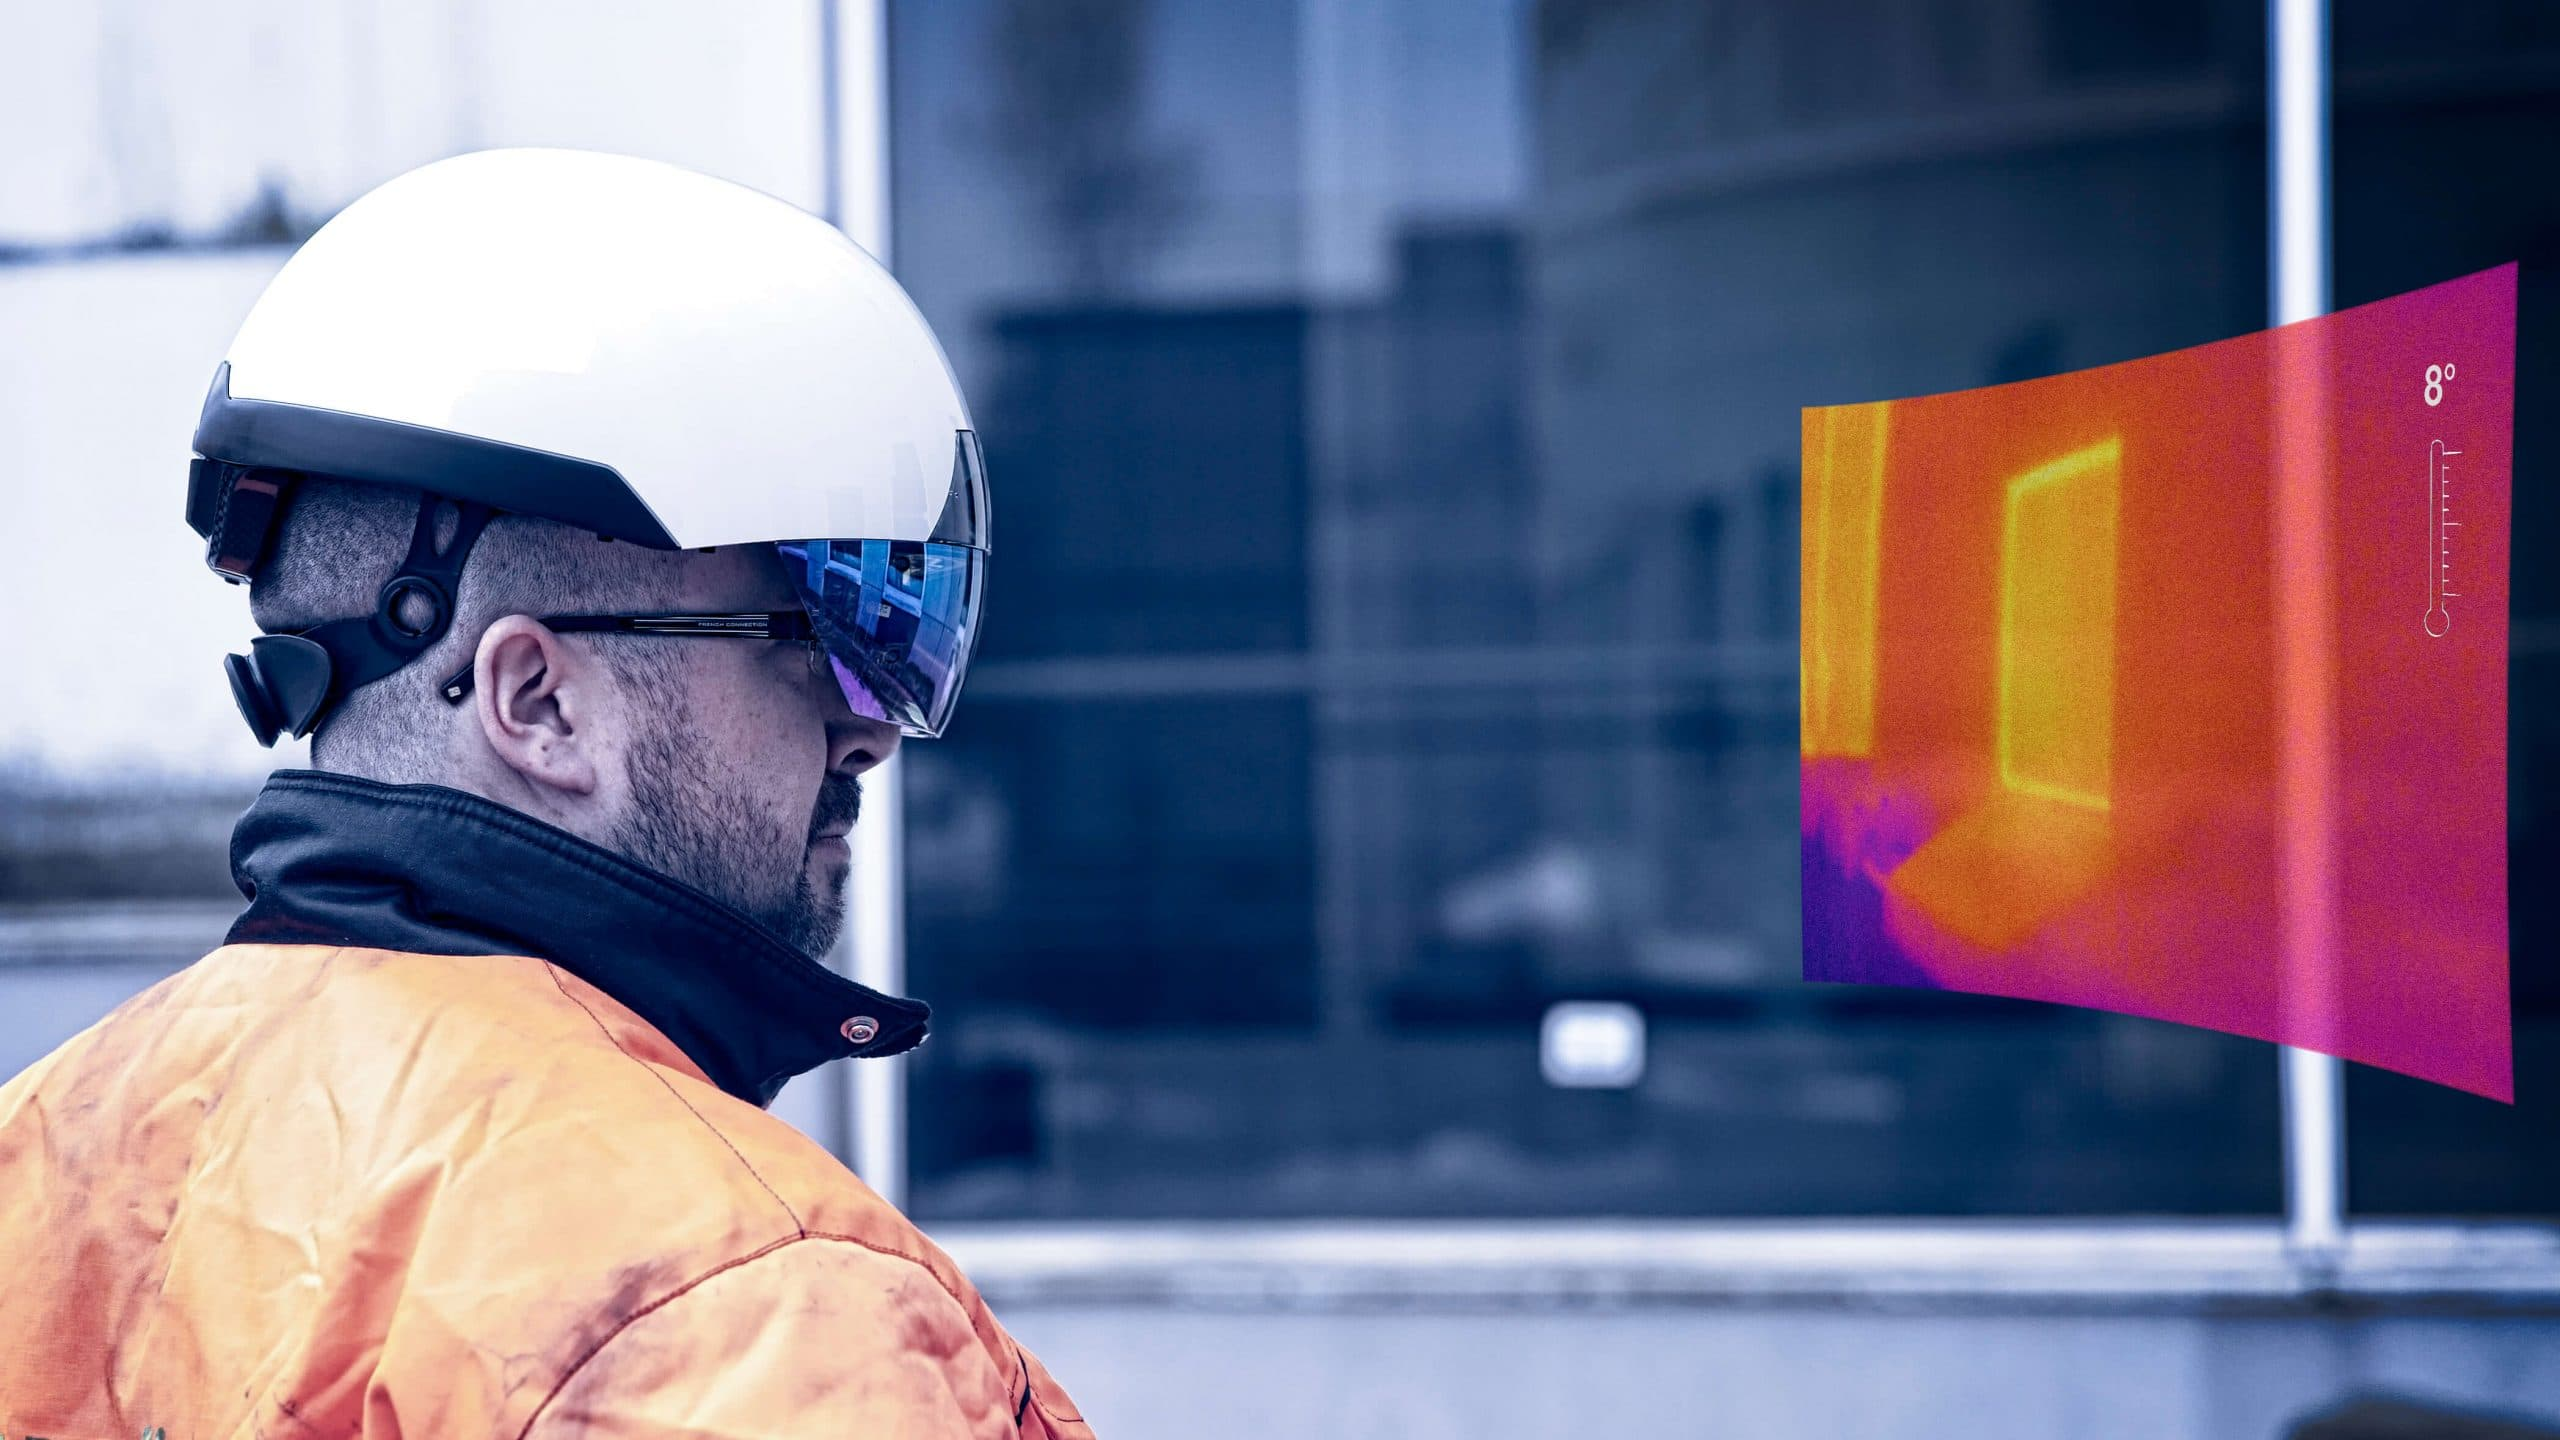
\includegraphics[width=0.3\textwidth]{figures/daqri.jpg}
	\rule{0.3\textwidth}{0.5pt} % use line???
	\caption[The Daqri Smart Helmet.]{The Daqri Smart Helmet \citep{DAQRI:stereoscape}.}
	\label{fig:daqri}
\end{wrapfigure}

I also have an appreciation of likely new developments, thanks to \ICPTitle.
This includes the use of virtual and augmented reality,
robotics,
modern methods of construction (MMC),
smart helmets (see Figure~\ref{fig:daqri}),
localisation and identification technologies (e.g. Global Navigation Satellite System (GNSS) and radio-frequency identification (RFID))
in construction.







\subsection*{P10m} \label{sec:P10m}

\begin{wraptable}{r}{0.2\textwidth}
    \begin{tabular}{|ll|}
        \hline
        \multicolumn{2}{|c|}{\cellcolor[HTML]{F8A102}\textbf{P10(i, b, m)} \littlemaster} \\ \hline
        \multicolumn{2}{|c|}{\PRJ} \\ \hline
    \end{tabular}
\end{wraptable}

I have on one occasion applied engineering techniques while taking account of commercial and industrial constraints.
During the 4\textsuperscript{th} year collaborative project (part of \PRJ), I used inspiration from the proposed Swansea Bay Tidal Lagoon in South West Wales to suggest a way to generate tidal power on our building site
(see a video demonstrating the tidal lagoon concept here: \url{http://www.tidallagoonpower.com/projects/swansea-bay/3d-model/}).
As I was researching the tidal technology, I discovered that the hydro turbines needed to be bi-directional (i.e. work in reverse) in order to take advantage of both the ebb and flood tides \citep{TurbineTech}, but that such turbines were not readily available on the market. 
%\hl{(source cannot currently be found).}
Therefore my group allocated a substantial amount of the budget to the manufacture of custom turbines, such as by Andritz Hydro \citep{TurbineTech}.

%I also attempted to study the viability of tidal power generation at the building site by calculating the potential annual yield of a tidal lagoon set-up.
%Because this is a fairly new technology, I struggled to find calculation methods.
%I eventually had to make assumptions and I used a yield equation for hydroelectricity (? \hl{find calcs and scan in!}).

This is the only example I can think of that demonstrates my achievement (if partial) of P10m.
Since it is a Masters level LO, I will hopefully get opportunities to further develop this ability in Semester 2 of Year 5, or when I start to work in industry.





\subsection*{P11(i, b, m)}

% Similar to G4

\begin{wraptable}{r}{0.2\textwidth}
    \begin{tabular}{|ll|}
        \hline
        \multicolumn{2}{|c|}{\cellcolor[HTML]{F8A102}\textbf{P11(i, b, m)} \nomaster} \\ \hline
        \CAS & \TPS \\
        \PRJ & \LAB \\
        Arup & Hoare Lea \\
        \multicolumn{2}{|l|}{Hultin \& Lundquist} \\ \hline
    \end{tabular}
\end{wraptable}

Every year, my ability to work as a team member in the role of an architectural engineer has increased, as has my awareness of the team roles of a building design team (a type of engineering team) [\textbf{P11i}].
This is thanks to my involvement in almost annual cross-disciplinary design projects, notably the 2\textsuperscript{nd} year and 4\textsuperscript{th} year collaborative projects, and the design project in \CASTitle, and my attendance at design team meetings at some of my placements.
The roles of a building design team include:
\begin{itemize}
    \item Urban planners, who look at the overall socio-economic aspects of urban development and consider the benefits and viability of constructing a building in a certain area
    \item Quantity surveyors, who calculate the costs of a building project
    \item Structural and civil engineers, who design the sub- and superstructure of a building, ensuring the whole structure is supportive and resilient
    \item Architectural engineers (a.k.a. building services engineers), who make the building usable and comfortable, and whose work greatly influences the operational energy consumption and costs
    \item Interior designers, who style the building interior
    \item Construction project managers, who supervise and coordinate the efforts of the construction workers on site
\end{itemize}


\begin{figure}[htbp]
	\centering
	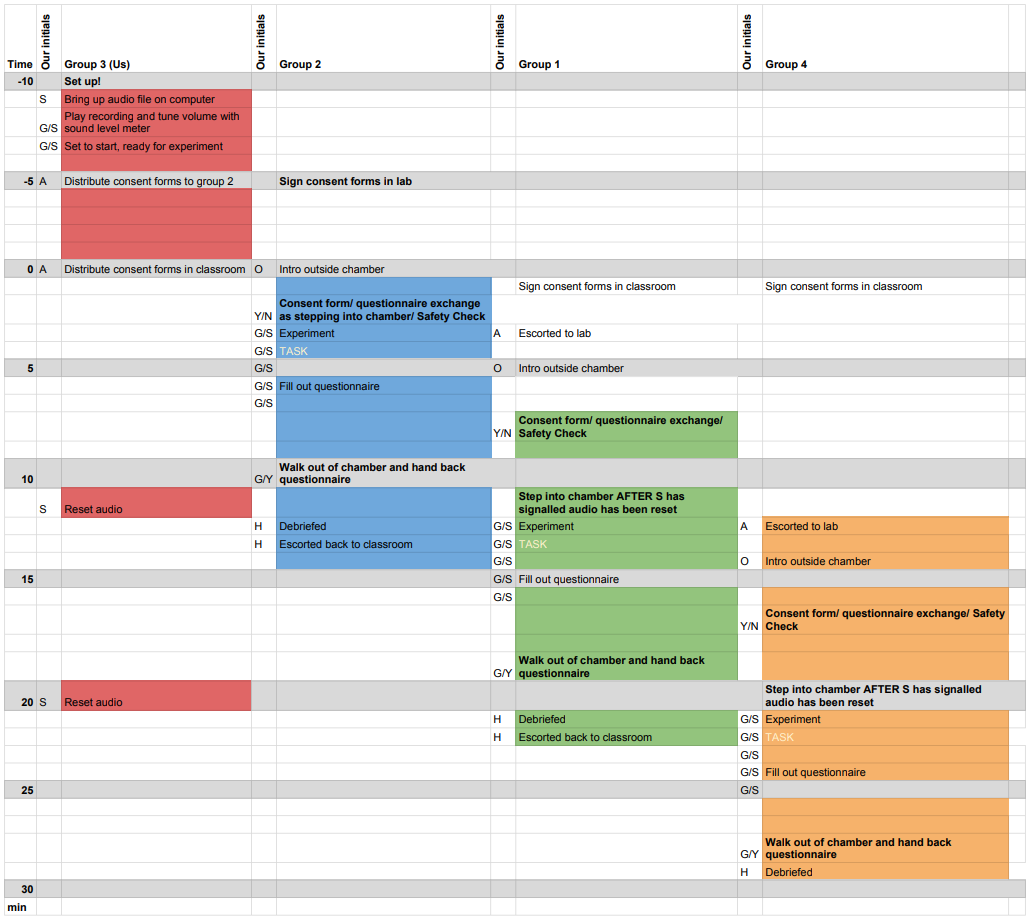
\includegraphics[width=0.5\textwidth]{figures/lab-gantt.PNG}
	\rule{\textwidth}{0.5pt} % use line???
	\caption[Acoustics experiment programme.]{The programme I created to coordinate my group in an acoustics laboratory experiment (\LAB).}
	\label{fig:lab-gantt}
\end{figure}



My ability to exercise personal responsibility as a member of an engineering team can be demonstrated by my contribution to the passive design (e.g. natural lighting) of a library building, which helped our group win the 1\textsuperscript{st} prize in sustainability in \CASTitle \space (see Figure~\ref{fig_award}).

Apart from AE, the only other team role I may have a partial understanding of is that of the project manager.
This is due to my frequent experiences of leading and coordinating a team in group projects,
%\hl{(example?)}, 
as well as my self-initiated attempts to use a Gantt-\textit{esque} chart to plan the timeline of a group-conducted acoustics experiment in \LABTitle \space (see Figure~\ref{fig:lab-gantt})
and
my dissertation work (see Figure~\ref{DST_schedule}) [\textbf{P11b and P11m}].

Unfortunately, I have not come as far as to understand the other aforementioned roles of a building design team.
This is because I have not had experience using my knowledge (albeit limited) of those roles.
Regarding quantity surveying, I have had at least two opportunities to try out that role (in the \CASTitle \space design project and the \PRJTitle), but I did not use these opportunities.
Another opportunity I missed that may have improved my understanding of some of these roles is \textit{Constructionarium}, a week-long, on-site and hands-on construction project where a team of students replicate an existing structure (e.g. a tower or bridge) in miniature scale.
%----------------------------------------------------------------------------------------
%	SECTION 6
%----------------------------------------------------------------------------------------

\section{Additional General Skills (G)}


\subsection*{G1} \label{sec:G1}

% Please add the following required packages to your document preamble:
% \usepackage[table,xcdraw]{xcolor}
% If you use beamer only pass "xcolor=table" option, i.e. \documentclass[xcolor=table]{beamer}
\begin{wraptable}{r}{0.2\textwidth}
	\begin{tabular}{|c|}
		\hline
		\rowcolor[HTML]{F8A102}
		\textbf{G1} \master \\ \hline
		All courses and \\
		placements \\ \hline
	\end{tabular}
\end{wraptable}

I have had several opportunities to apply my skills in problem solving, communication, information retrieval, working with others and the effective use of general IT facilities.
I will demonstrate my application of these skills by providing examples from the work I produced for Sunamp and \textit{Climate Change, Sustainability and Adaptation} (\CCSA).
%A good example is when I applied these skills to produce the UniQ Overview Sheet, Product Selection Quiz and PISs for Sunamp (see \Cref{App:Overview,App:quiz,App:PISs}).
I applied my skills in:
\begin{itemize}
    \item Problem solving at Sunamp, as demonstrated in Section \ref{sec:quiz}, by solving the problem of guiding customers to their most suitable UniQ products through the creation of a quiz (see Appendix~\ref{App:quiz}).
    %when I encountered inconsistencies or unclear information in the UniQ manuals.
    %For example, I was tasked with providing accurate and up-to-date dimensions of the UniQ batteries because the dimensions provided in the UniQ manuals were inconsistent.
    %Therefore, I asked a staff member what might be the cause for the discrepancy and they explained that the different dimensions might be referring to different UniQ prototypes.
    %They also suggested that I measure the batteries that were currently being mass-produced.
    %So I asked for a tape measure and used it to measure the dimensions of the most current UniQ batteries.
    %I also cross-checked my measurements with the staff member's until we settled on reasonable nominal dimensions.
    %As a result, I created a diagram with the nominal dimensions... 
    
    \item Communication during a recent D11CA assignment in which the aim was to write a POSTnote.
    POSTnotes are briefings on public policy issues that are based on academic and industrial research.
    They are written to inform the Parliamentary Office of Science and Technology (POST) so that appropriate policies can be developed.
	The crux of the assignment was to write technical information in layman's terms so that any politician could fully understand the issue at hand before entering a parliamentary debate or meeting.
	I wrote my POSTnote on adapting UK households to a 2050 climate and received a provisional mark of 67\%.
	My communication was successful, as my feedback reflects:
	``Overall, this is very clearly written and easy to understand."
    %as I produced the documents.
    %With the development of the quiz, I managed to come up with a way to efficiently direct customers to the most suitable UniQ product for them, which made the customers more informed and reduced the workload for the sales team.
    
    \item Information retrieval at Sunamp in order to produce accurate PISs (see Appendix~\ref{App:PISs}).
    This was done by reading the UniQ manuals and other documents, doing online research and asking staff members for explanations to fill my gaps in understanding, and hands-on experience (e.g. measuring the dimensions of UniQ batteries).
    
    \item Working with others at Sunamp in order to produce the UniQ documents, which was a collaborative effort.
    (See Sections \ref{sec:quiz} and \ref{sec:piss} for references to collaborations and iterative feedback processes.)
    
    \item The effective use of general IT facilities at Sunamp throughout the production of the UniQ documents.
    For example, I would regularly print out my latest drafts for easy marking-up during meetings and back up my drafts online on Google Drive.
    I also applied this skill in D11CA by converting a Word document (docx) to a Portable Document Format (pdf) so that the POSTnote could be displayed consistently over different IT systems.
    %utilised media conversion techniques to ensure that the same message was displayed consistently over different IT systems
    % I created the Overview Sheet on Microsoft Publisher, the quiz on Microsoft PowerPoint, and the PISs on Microsoft Word. % MS applications are just software, not facilities.
\end{itemize}



\subsection*{G2}

\begin{wraptable}{r}{0.2\textwidth}
    \begin{tabular}{|ll|}
        \hline
		\rowcolor[HTML]{F8A102}
        \multicolumn{2}{|c|}{\textbf{G2} \nomaster} \\ \hline
        \ConTechTwo & \HYD \\
        \DPB & \CAS \\
        \DSA & \PC \\
        \EnBldgs & \TPS \\
        \DI & \PRJ \\
        \DST & \LAB \\
        \IP & \CCSA \\
        Arup & Hoare Lea \\
        Sunamp & Sweco \\
        \multicolumn{2}{|l|}{Hultin \& Lundquist} \\ \hline
    \end{tabular}
\end{wraptable}

\textit{N.B. For this LO, I have interpreted ``self-learning" as ``self-initiated learning", i.e. 
myself deciding and taking action to learn something that is not mandated by an external force,
%OR myself taking the initiative to learn something
whether I teach it to myself or somebody else teaches it to me.}

During my years at Heriot-Watt University, I have not initiated a personal project with the aim of learning something within a certain time frame.
Hence, I have not \emph{planned self-learning and improved performance} within a single project.
I would still consider myself to be a lifelong learner, though, as I have planned my self-learning and improved my performance on separate occasions.

%On the one hand, my personal programme of work that I used during my Dissertation (see Figure~\ref{DST_schedule}) demonstrates my ability to plan self-learning.
%Moreover, my strategic approach to selecting optional courses and applying for placements demonstrates my ability to plan self-learning.
%in order to gain the most interesting and relevant knowledge to my course and gain exposure to different fields of work

On the one hand, my ability to \emph{plan self-learning} can be demonstrated by my personal programme of \DST \space work (see Figure~\ref{DST_schedule}), as well as my strategic approach to selecting optional courses and applying for placements.
In Year 2, I selected \HYD \space and \DPB \space as I thought they would respectively deepen and develop my Architectural Engineering knowledge and design skills.
Since Year 2, also, I have tried to gain exposure to different fields of work through my summer placements.
Thus, I have so far experienced working in Mechanical Engineering, Architecture, Electrical Engineering, Environmental Building Certification, and Renewable Energy.

\begin{wrapfigure}{r}{0.4\textwidth}
	\centering
	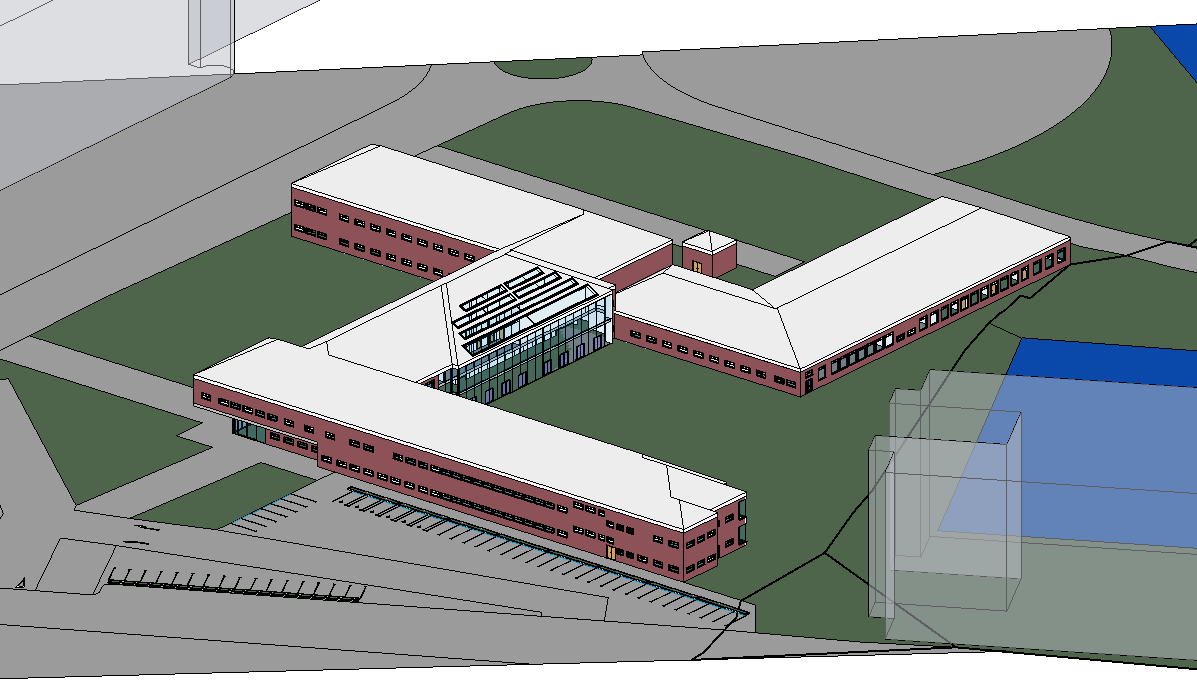
\includegraphics[width=0.4\textwidth]{figures/South.PNG}
	\rule{0.4\textwidth}{0.5pt} % use line???
	\caption{The building model I created in Revit for the \PRJTitle.}
	\label{fig:revit}
\end{wrapfigure}

On the other hand, I have self-learned to \emph{improve my performance} in certain IT skills, notably modelling in Revit and writing documents in LaTeX.
During the \PRJTitle, I attended Revit workshops that are provided on a weekly basis by the \deptname.
%(EGIS).
This learning experience improved my Revit modelling skills, enabling me to produce a building model for the \PRJTitle \space (see Figure~\ref{fig:revit}).
As for LaTeX, since I was introduced to the document preparation system in Year 2, I have written most of my assignments in the system.
This has improved my ability to produce large professional-looking documents with reduced formatting-hassle (a problem I often experienced in Microsoft Word).
This report, for example, was written in LaTeX.




\subsection*{G3(i, b, m)}

\begin{wraptable}{r}{0.2\textwidth}
    \begin{tabular}{|ll|}
        \hline
        \rowcolor[HTML]{F8A102}
        \multicolumn{2}{|c|}{\textbf{G3(i, b, m)} \nomaster} \\ \hline
        \PRJ & \ISE \\
        \DST & \SIB \\
        \LAB & \ICP \\
        \multicolumn{2}{|c|}{Sunamp} \\ \hline
    \end{tabular}
\end{wraptable}

Throughout my years at Heriot-Watt University, I have increasingly planned and carried out a personal programme of work.
This culminated in Year 4, when we had the \textit{Design Project} and \textit{Dissertation} which were both long-term personal projects.
In the interim report that I wrote for my Dissertation, I included a personal programme of work (similar to a Gantt chart) that mapped out when and how I would work on the different sections of my dissertation for the rest of the academic year (see Figure~\ref{DST_schedule01}).
I \emph{adjusted} the programme as I carried it out (see final programme in Figure~\ref{DST_schedule02}) [\textbf{G3b}].
The major variations between the initial and final versions of the programme are:
\begin{itemize}
    \item No more work was done in Semester 1 and during the Christmas holidays. This was because I had decided that it was better for me to use that time to focus on my Design Project instead.
    \item The programme was more compressed, due to the above reasons.
    \item The blue block was segmented into two blocks. Blue represented my work on questionnaires and interviews. The gap was introduced to allow the respondents time to answer my survey before I interviewed them.
\end{itemize}

%\hl{Whereas I mostly assisted my supervisors with their projects at my other placements, the work I did at Sunamp was very much a personal project....}


\begin{figure}[htbp]
    \centering
        \begin{subfigure}{.45\textwidth}
          \centering
          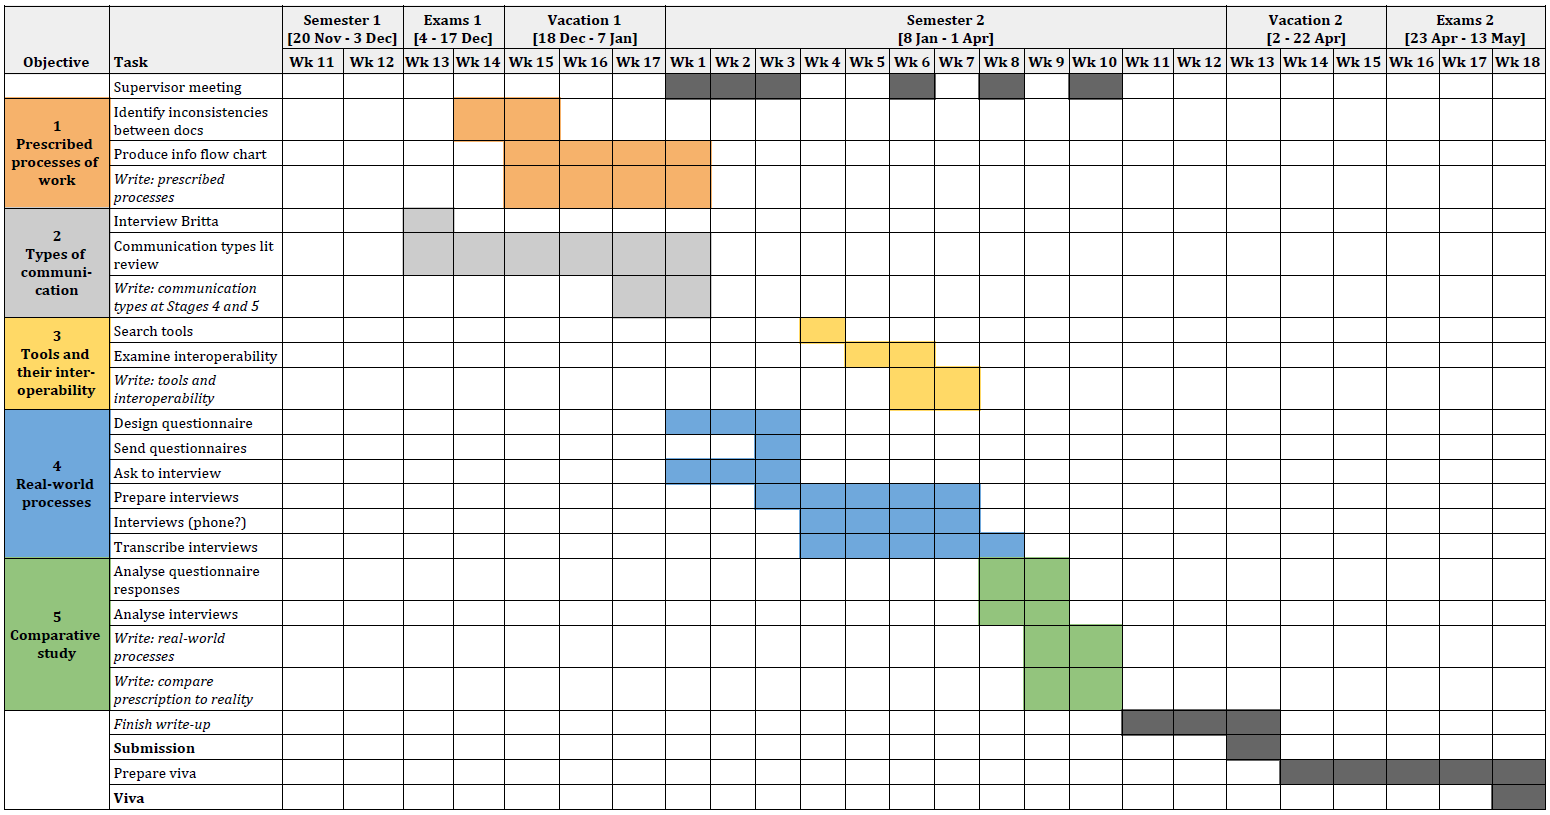
\includegraphics[width=\textwidth]{figures/DST-schedule-start.PNG}
%          \rule{\textwidth}{0.5pt} % use line???
          \caption{Initial programme}
          \label{DST_schedule01}
        \end{subfigure}
        \begin{subfigure}{.51\textwidth}
          \centering
          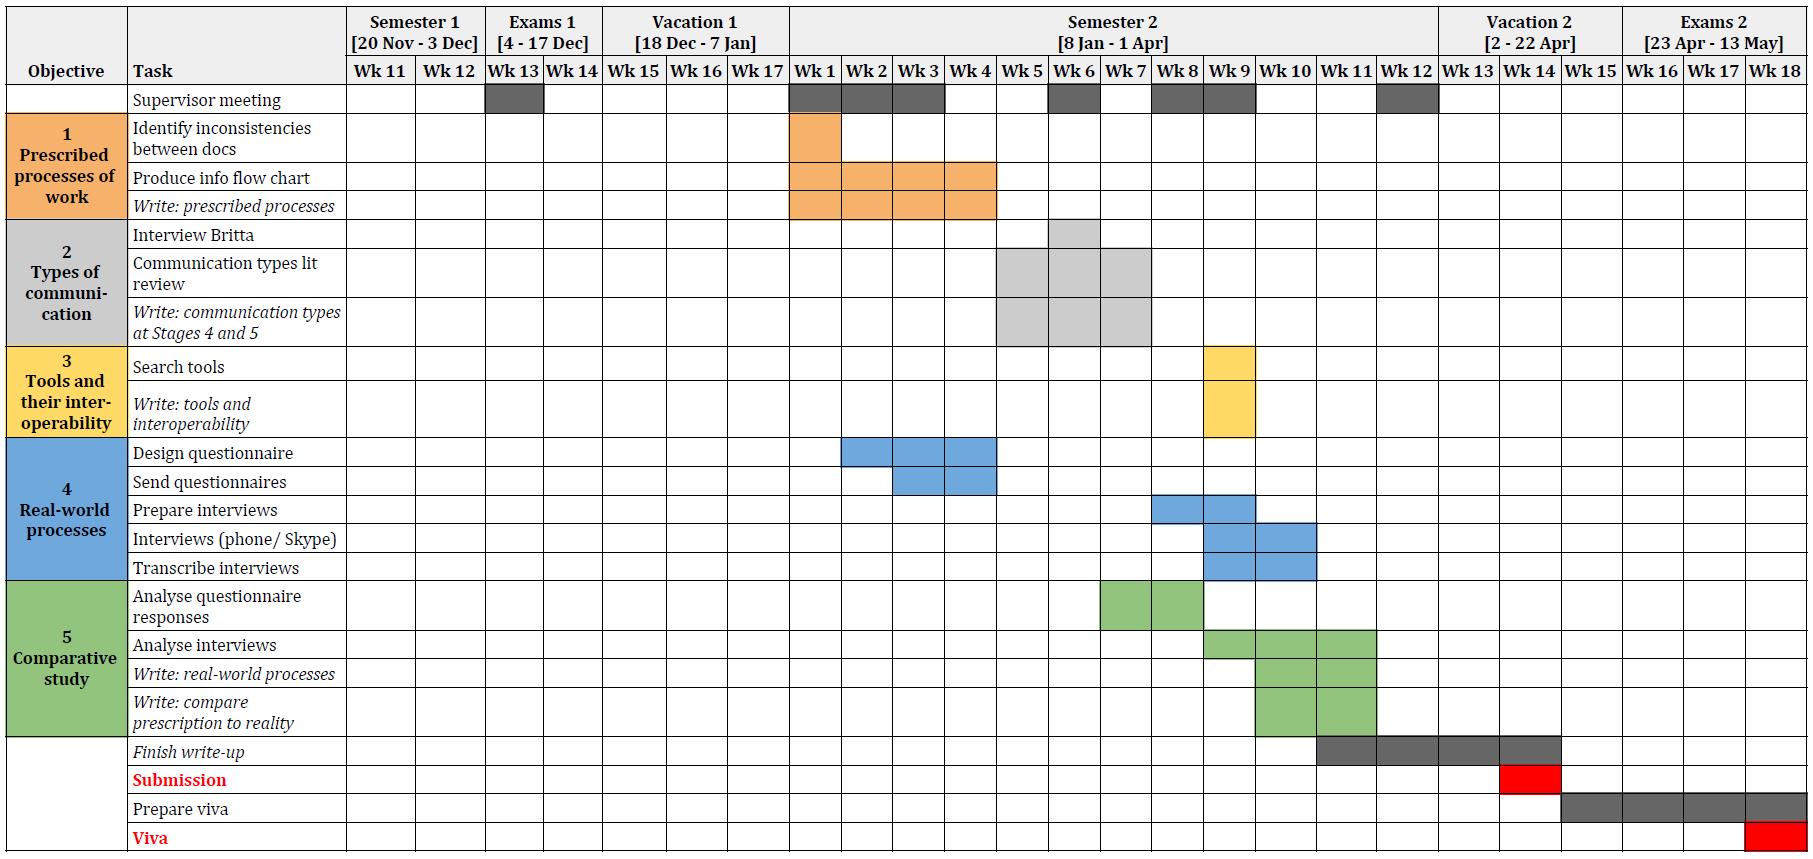
\includegraphics[width=\textwidth]{figures/DST-schedule-end-big.PNG}
%          \rule{\textwidth}{0.5pt} % use line???
          \caption{Final programme}
          \label{DST_schedule02}
        \end{subfigure}
    \rule{\textwidth}{0.5pt} % use line???
    \caption[My personal programme of work for my dissertation.]{My personal programme of work for my dissertation, from the end of Semester 1 to to the end of Semester 2 of Year 4.}
    \label{DST_schedule}
\end{figure}


\begin{wrapfigure}{r}{0.5\textwidth}
	\centering
	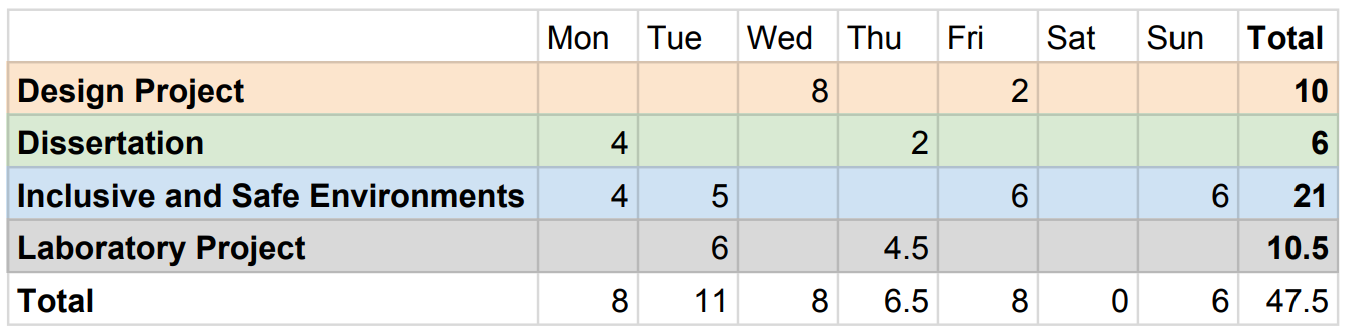
\includegraphics[width=0.5\textwidth]{figures/y4s1w6hours.PNG}
	\rule{0.5\textwidth}{0.5pt} % use line???
	\caption{Time log from Week 6 of Semester 1, Year 4.}
	\label{fig_timelog}
\end{wrapfigure}

In Year 4, I also started to \emph{monitor} the hours I worked in order to \emph{adjust} and improve my personal programme \emph{on an on-going basis} [\textbf{G3m}].
Figure~\ref{fig_timelog} provides an example of my weekly time log from Year 4.
By monitoring the hours I worked, I noticed a trend: I typically worked fewer hours on Thursdays than any other day.
I proceeded to identify the reason for this, which is that I tended to feel tired or burnt out by that day of the week.
After this discovery, I allocated myself less hours to work and focused on less demanding tasks (if possible) on Thursdays.
The hours that I lost on Thursday I would then try to compensate for throughout the rest of the week.




\subsection*{G4(i, -)}

\begin{wraptable}{r}{0.2\textwidth}
    \begin{tabular}{|ll|}
        \hline
        \rowcolor[HTML]{F8A102}
        \multicolumn{2}{|c|}{\textbf{G4(i, -)} \master} \\ \hline
        \ID & \IE \\
        \EnvBeh & \CAS \\
        \EnBldgs & \TPS \\
        \DI & \FMP \\
        \PRJ & \LAB \\
        \ISE & \CCSA \\
        Arup & Hoare Lea \\
        Sunamp & Sweco \\
        \multicolumn{2}{|l|}{Hultin \& Lundquist} \\ \hline
    \end{tabular}
\end{wraptable}

My degree programme and my work placements have provided me with multiple opportunities to work as part of a team.
In all of the projects, I have exercised personal responsibility, and sometimes also initiative, as a team member.
For example, the work I produced for Sunamp, including the quiz I came up with (see Section \ref{sec:sunamp_work}), is a display of me exercising initiative and my personal responsibility to the company.

In most academic projects, however, I have exercised personal responsibility, and sometimes initiative, as a team leader.
% Sometimes this has involved me exercising initiative also.
A recent example of this is a group project of creating and presenting a poster for \textit{Climate Change, Sustainability and Adaptation}.
I assumed a leading role in this group mainly by coordinating the group activity (e.g. arranging and leading meetings, setting up weekly agendas).
For this project, I sketched the drawing in Figure~\ref{fig:Sketch01} and suggested the use of such an image to graphically show the importance of our topic.
After the group agreed on its usefulness to the poster, I went ahead and developed a final version (see Figure~\ref{fig:Sketch02}).
This was an act of initiative because the use of a representative image had previously not been discussed within the group.


\begin{figure}[htbp]
    \centering
        \begin{subfigure}{.49\textwidth}
          \centering
          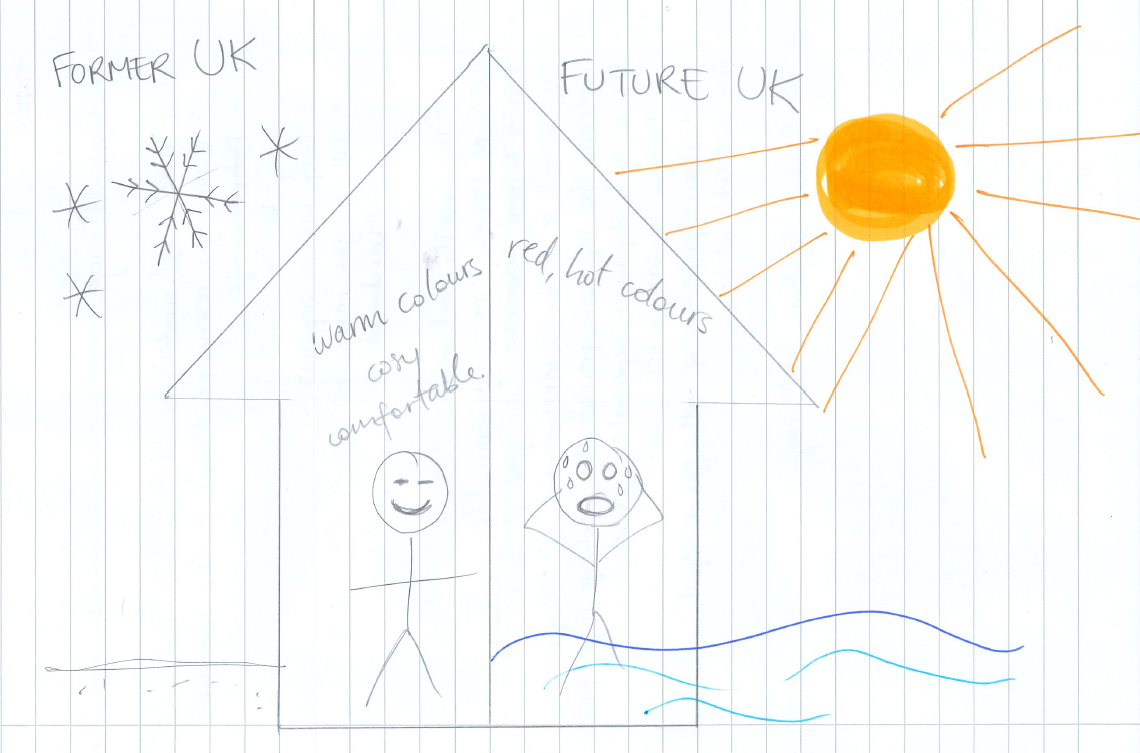
\includegraphics[width=\textwidth]{figures/sketch.PNG}
%          \rule{\textwidth}{0.5pt} % use line???
          \caption{Initial sketch}
          \label{fig:Sketch01}
        \end{subfigure}
        \begin{subfigure}{.47\textwidth}
          \centering
          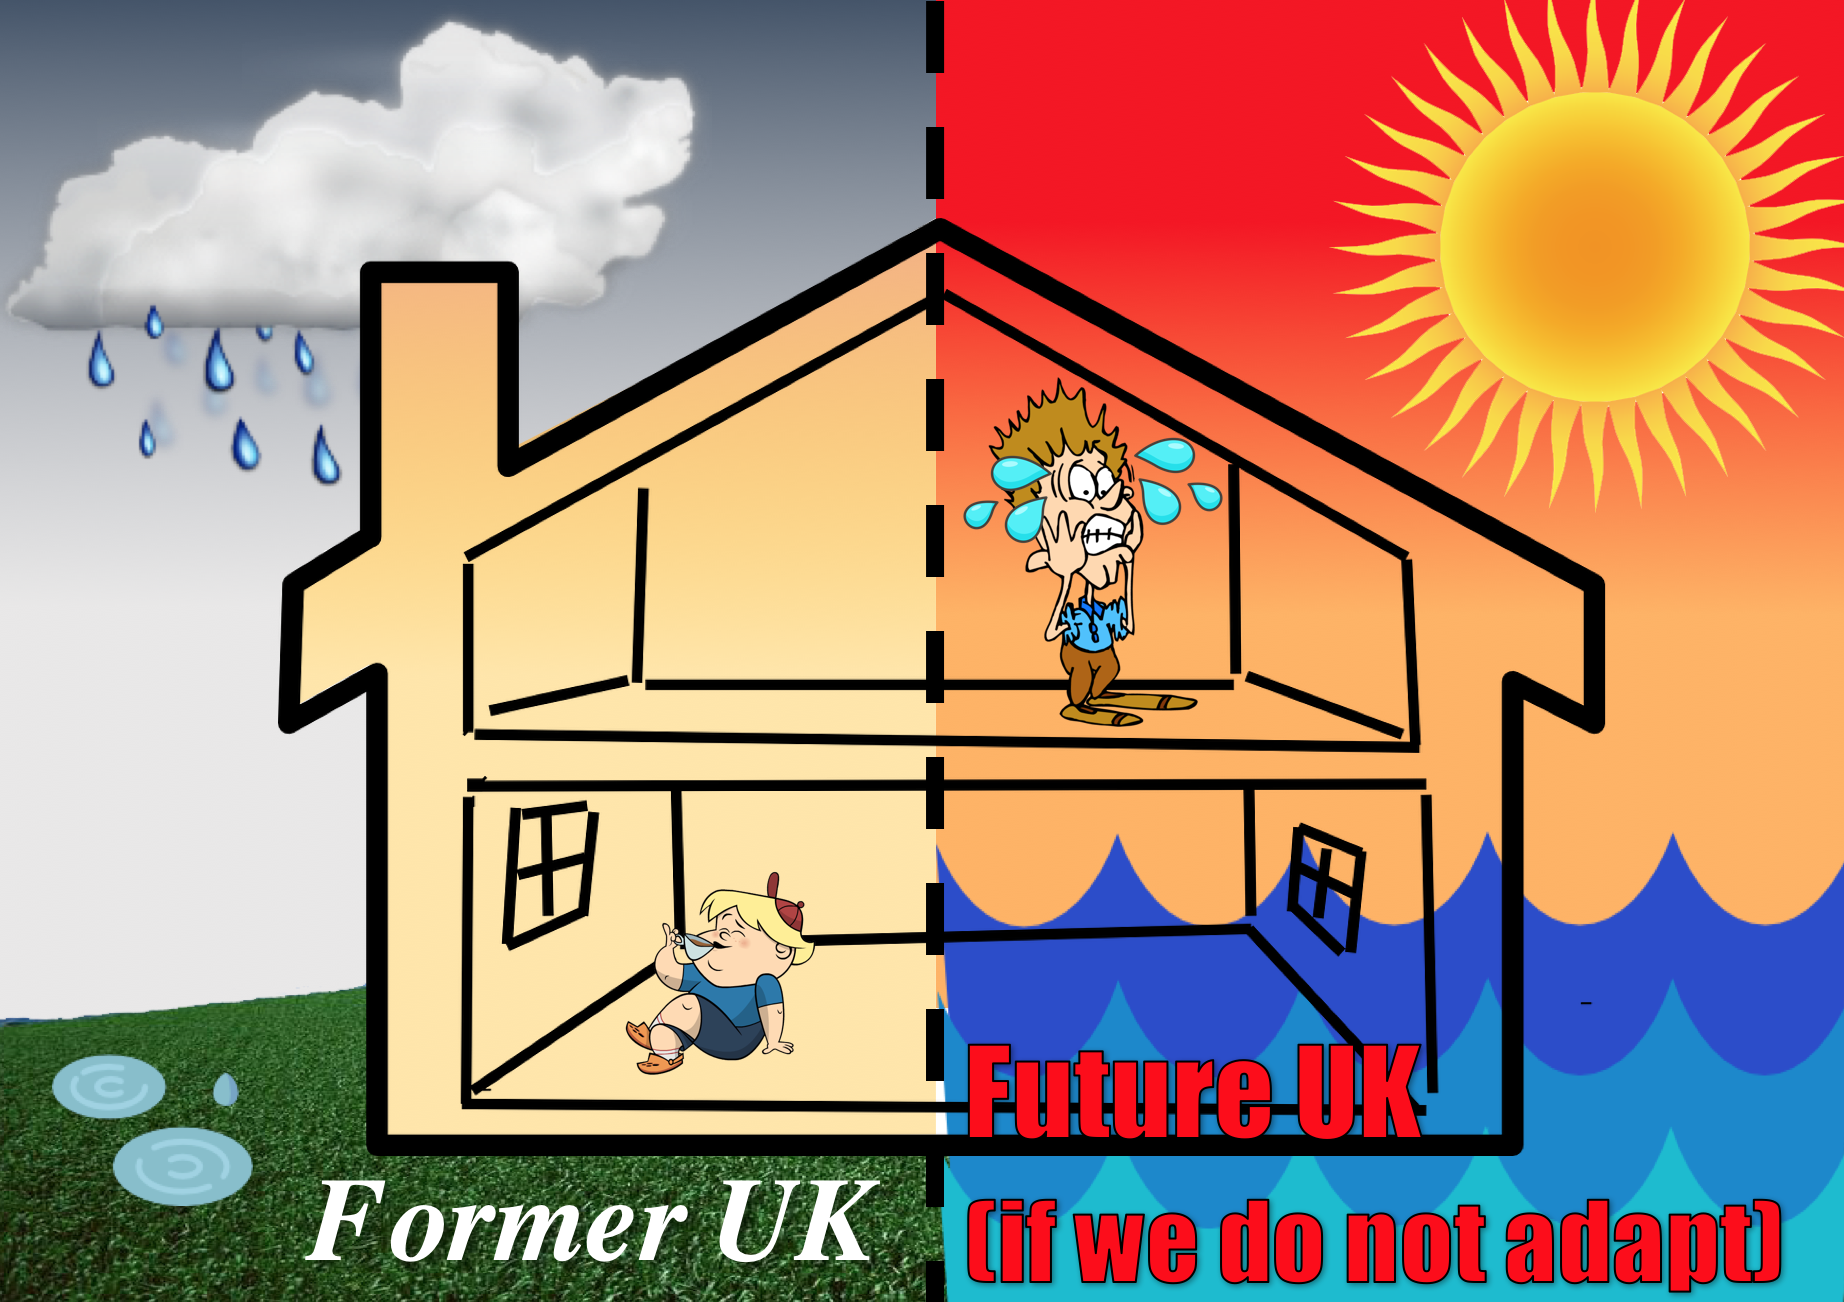
\includegraphics[width=\textwidth]{figures/eposter_sketch_2.png}
%          \rule{\textwidth}{0.5pt} % use line???
          \caption{Final image}
          \label{fig:Sketch02}
        \end{subfigure}
    \rule{\textwidth}{0.5pt} % use line???
    \caption[\CCSA poster image.]{The image I suggested and developed to use on a group poster to show the importance of adapting UK houses to future climate impacts.}
    \label{fig:Sketch}
\end{figure}

